\documentclass[russian,utf8,pointsection]{eskdtext}
\usepackage{cmap}			% Поиск по русским словам в конечном pdf документе
\usepackage{eskdchngsheet}
\usepackage[T2A]{fontenc}
\usepackage{pscyr}			% Подключение "красивых" шрифтов киррилицы
\usepackage{amstext}
\usepackage{amsmath}
\usepackage{listings}
\usepackage{tablefootnote}

\usepackage{listings}		
\lstset{ %
	language=tcl,           % Язык программирования 	
	frame=single,           % Добавить рамку
	breaklines=true,        % Автоматический перенос строк
	breakatwhitespace=true, % Переносить строки по словам
	title=\lstname 
}

% нумерация таблиц и рисунков по разделам
\usepackage{chngcntr}
\counterwithin{figure}{section}
\counterwithin{table}{section}


% работа с сылками
\usepackage{hyperref}
\usepackage[usenames,dvipsnames,svgnames,table,rgb]{xcolor}
\hypersetup{			
	unicode=true,           							% русские буквы в раздела PDF
	pdftitle={Руководство по эксплуатации (часть 2)},	% Заголовок
	pdfauthor={Щеблыкин М.В.},      					% Автор
	pdfsubject={Интерфейс <<Человек-машина>>},			% Тема
% 	pdfcreator={Latex},			 						% Создатель
% 	pdfproducer={Производитель}, 						% Производитель
% 	pdfkeywords={keyword1} {key2} {key3}, 	% Ключевые слова
	colorlinks=true,      					% false: ссылки в рамках; true: цветные ссылки
	linkcolor=NavyBlue,        				% внутренние ссылки
	citecolor=black,        				% на библиографию
	filecolor=black,        				% на файлы
	urlcolor=black          				% на URL
}

% Дает доступ к командам:
% \MakeTextUppercase{} - сделать все символы заглавными
\usepackage{textcase} 

%Изменение отображения Содержания
%\makeatletter
%\renewcommand{\l@section}{\@dottedtocline{1}{0em}{1.25em}}
%\renewcommand{\l@subsection}{\@dottedtocline{2}{1.25em}{1.75em}}
%\renewcommand{\l@subsubsection}{\@dottedtocline{3}{2.75em}{2.6em}}
%\makeatother

% Работа с таблицами
% p{} - top align, m{} - middle align, b{} - bottom align
\usepackage{ltablex} 										% longtable с функциональностю tabularx
\usepackage{multirow} 										% Слияние строк в таблице
\renewcommand{\tabularxcolumn}[1]{>{\arraybackslash}m{#1}}	% выравнивание в ячейке таблицы по середине по вертикали
\newcolumntype{M}[1]{>{\centering \arraybackslash}m{#1}} 	% колонка с заданной шириной и выравниванием по центру
\newcolumntype{Z}{>{\centering \arraybackslash} X} 			% колонка с выравниванием по центру
\newcolumntype{L}{>{\raggedright\arraybackslash} X} 		% for ragged-right material
\newcolumntype{C}{>{\centering\arraybackslash} X} 			% for centered material

% Добавлено отображение Города на Титульном листе
\renewcommand{\ESKDtheTitleFieldX}{Екатеринбург \\ \ESKDtheYear}

% Уменьшен размер шрифта для заголовков секций
\ESKDsectStyle{section}{\large \bfseries \MakeTextUppercase}

% Выравнивание по центру.
% Предназначено для выравнивания надписей в шапке таблицы
\newcommand{\calign}[1]{\centering #1 \arraybackslash} 

%%% Работа с картинками
\usepackage{graphicx}  			% Для вставки рисунков
\graphicspath{{images/}}  		% папки с картинками
\setlength\fboxsep{3pt} 		% Отступ рамки \fbox{} от рисунка
\setlength\fboxrule{1pt} 		% Толщина линий рамки \fbox{}
\usepackage{wrapfig} 			% Обтекание рисунков и таблиц текстом
\usepackage{float}

%%% Информация
\newcommand{\info}[1]{ %
\begin{flushleft}%
	\begin{tabular*}{\linewidth}{m{0.05\linewidth}m{0.9\linewidth}}%
		\includegraphics[width=\linewidth]{info.jpg} & \textcolor{ForestGreen}{\textit{#1}}
	\end{tabular*}	
\end{flushleft}	
}

%%% Предупреждение
\newcommand{\warning}[1]{ %
\begin{flushleft}%
	\begin{tabular*}{\linewidth}{m{0.05\linewidth}m{0.9\linewidth}}%
		\includegraphics[width=\linewidth]{warning.png} & \textcolor{Red}{\textit{\textbf{#1}}}
	\end{tabular*}	
\end{flushleft}	
}

%%% Переопределение отображения счетчиков enumerate на отображение цифрами
\renewcommand{\theenumi}{\arabic{enumi}}
\renewcommand{\labelenumi}{\theenumi)}

\usepackage[backend=biber,bibencoding=utf8,sorting=ynt,maxcitenames=2,style=authoryear]{biblatex}
\addbibresource{bib_orcad.bib}

%%% используется для рисования
\usepackage{tikz}
\usetikzlibrary{trees}

%\usepackage{ragged2e}

%%% Используется для изменения направления текста
\usepackage{rotating}

\usepackage{caption}

%%% Без куска ниже проект не собирается
\providecommand{\No}{\textnumero}
\makeatletter
\newsavebox\ESKDpicturebox
\renewcommand{\ESKD@ShipoutPicture}{%
     \ifESKD@twoside
       \ifodd\c@page
         \ESKDframeX=\ESKD@margin@si
       \else
         \ESKDframeX=\ESKD@margin@so
       \fi
     \else
       \ESKDframeX=\ESKD@margin@si
     \fi
     \ESKDframeY=\ESKD@margin@b
     \ESKDstampX=\ESKDframeX
     \advance\ESKDstampX \ESKDframeW
     \advance\ESKDstampX -185mm
     \ESKDstampY=\ESKDframeY    
     \sbox\ESKDpicturebox{%
        \unitlength=1mm
        \begin{picture}(0,0)(\ESKDltu{\ESKD@origin@x},\ESKDltu{\ESKD@origin@y})%
          \ifx\ESKD@thisstyle\@empty
            \let\ESKD@thisstyle\ESKD@curstyle
          \fi
          \loop
          \ifnum \ESKD@hash@pos{@style@draw@\ESKD@thisstyle} %
            < \ESKD@hash@count{@style@draw@\ESKD@thisstyle}
            \ESKD@hash@next@value{@style@draw@\ESKD@thisstyle}\relax
          \repeat
          \ifx\ESKD@extra@ThisHook\@empty%
            \ESKD@extra@Hook\else\ESKD@extra@ThisHook%
          \fi%
          \global\let\ESKD@thisstyle\@empty%
          \global\let\ESKD@extra@ThisHook\@empty%
        \end{picture}
        }%
       \AddToHook{shipout/foreground}{%
       \put(1in,-1in){\usebox\ESKDpicturebox}}%        
}

\makeatother


% Заполнение граф Титульного листа и основной надписи
\ESKDcompany{ООО <<Прософт-Системы>>}
\ESKDclassCode{ОКП 42 3211}
\ESKDtitle{ПРИЕМОПЕРЕДАТЧИК СИГНАЛОВ АВАНТ Р400}
\ESKDdocName{\vspace{0.5cm} Руководство по эксплуатации (часть 2) \\ Интерфейс <<Человек-машина>> 7v68}
\ESKDsignature{ПБКМ.42 4325.001 РЭ.01}
\ESKDgroup{\normalsize ООО <<Прософт-Системы>>}

% основная надпись
\ESKDauthor{\ESKDfontII Щеблыкин М.В.} 
\ESKDchecker{\ESKDfontII Кичигина Г.В.}
\ESKDnormContr{\ESKDfontII Бунина О.Ю.}
\ESKDapprovedBy{\ESKDfontII Чирков А.Г.}
\ESKDdate{2022/02/14}
\ESKDcolumnI{\ESKDfontIII{Приемопередатчик сигналов релейной защиты АВНАТ Р400} \\ \vspace{0.5cm} \ESKDfontIII{Рководство по эксплуатации (часть 2)}}

% Добавлено отображение Города на Титульном листе
\renewcommand{\ESKDtheTitleFieldX}{Екатеринбург \\ 2022}

% Уменьшен размер шрифта для заголовков секций
\ESKDsectStyle{section}{\large \bfseries \MakeTextUppercase}

\begin{document}
	\maketitle
	\tableofcontents  
	
	\newpage
	%%% ----------
\section{Панель управления и индикации блока БСП} \label{sec:overview}


%%% ----------
\subsection{Элементы панели управления и индикации}

Внешний вид панели управления и индикации показан на рисунке~\ref{fig:pi}.

\begin{figure}[H]
	\center{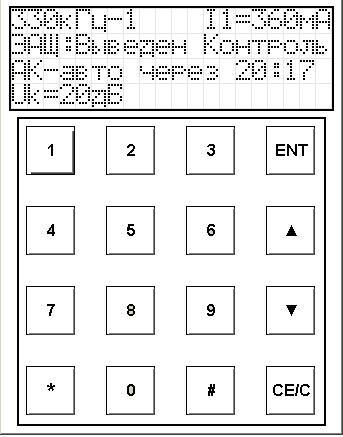
\includegraphics[width=0.4\linewidth]{pi.png}}
	
	\caption{Элементы панели управления и индикации}
	\label{fig:pi}
\end{figure}

Вывод информации в Р400 организован с помощью жидкокристаллического индикатора имеющего 4 строки по 20 символов. Управление осуществляется посредством 16-кнопочной клавиатуры. Информация на экране обновляется раз в секунду.


%%% ----------
\subsection{Индикация} 


%%% ----------
\subsubsection{Размещение информации в поле индикатора}

Индикатор условно разбит на 5 зон, как показано на рисунке~\ref{fig:overview_ind}.

\begin{figure}[H]
	\centering
	
	\begin{tabular}{| M{2.5cm} | M{2.5cm} |}	
		\firsthline
	    0 зона	& 1 зона 				\tabularnewline \hline 
	    \multicolumn{2}{|c|} {2 зона}	\tabularnewline \hline
	    \multicolumn{2}{|c|} {3 зона}	\tabularnewline \hline
	    \multicolumn{2}{|c|} {4 зона}	\tabularnewline 
	    \lasthline 
	\end{tabular} 
	
	\caption{Схемотичное расположение зон на индикаторе} 
	\label{fig:overview_ind}
\end{figure}

Информация, отображаемая в каждой зоне, представлена с сокращениями и, как правило, имеет законченный вид. Далее, по тексту, приводятся пояснения принятых сокращений и месторасположение сообщений по зонам.

Один из вариантов внешнего вида индикатора в исходном (нулевом) уровне показан на рисунке~\ref{fig:overview_level0}. 

\begin{figure}[H]
	\centering
	
	\begin{tabular}{| m{2.5cm}  m{2.5cm} |}
		\firsthline
		330кГц	& \raggedleft I1=360мА 				\tabularnewline 
		\multicolumn{2}{|l|} {ЗАЩ:Выведен Контроль}	\tabularnewline 
		\multicolumn{2}{|l|} {АК-авто через 20:17}	\tabularnewline 
		\multicolumn{2}{|l|} {Uk=20дБ}				\tabularnewline
		\lasthline
	\end{tabular} 
	
	\caption{Исходный (нулевой) уровень меню}
	\label{fig:overview_level0}
\end{figure}

0~зона предназначена для вывода информации о текущей дате (Число.Месяц.Год), времени (Часы.Минуты.Секунды) или частоты и номера аппарата (Частота-Номер). Выбор отображаемой информации осуществляется нажатием кнопок \textbf{[4]}~(предыдущий) и \textbf{[6]}~(следующий).

1~зона предназначена для вывода измерений. Листание параметров осуществляется кнопками \textbf{[2]}~(вверх) и \textbf{[8]}~(вниз).

Во 2-ой зоне в нулевом уровне выводятся сообщения, отражающие текущее состояние приемопередатчика сигналов защит (<<ЗАЩ>>), а также сообщения о типе неисправности или предупреждения.

При появлении события, вызывающего предупреждение, информация о текущем состоянии кратковременно, раз в секунду, подменяется соответсвующим сообщением.

В 3-ей зоне выводится тип автоконтроля и время до следующей проверки канала.

В 4-ой зоне всегда показывается уровень контрольной частоты, измеренный при последнем циле проверки канала.

При появлении события, вызывающего сообщение о неисправности (авария), информация о текущем состоянии или предупреждении заменяется аварийной.

Если неисправностей несколько, отображается сообщение старшее по приоритету.


%%% ----------
\subsubsection{Информация о текущем состоянии}

Вид сообщений, отражающих текущее состояние, показан в таблице \ref{tab:overview_reg}.

\begin{tabularx}{\linewidth}{| m{2.5cm} | X | p{11cm} |}
	\caption{Состояния и режимы работы <<ЗАЩ>>}  	\label{tab:overview_reg}	\tabularnewline

	\firsthline
	\centering Поле					& 
	\centering Показания индикатора	& 
	\centering Примечание	
	
	\tabularnewline \hline
	\multirow{ 2}{*}{Режим}	& Введен		&	\tabularnewline \cline{2-3}
							& Выведен		&	\tabularnewline \hline
	\multirow{ 7}{*}{Состояние} & Исходн	& Включение питания, инициализация. \tabularnewline \cline{2-3}
							& Контроль		& Контроль канала, нет сигналов <<Пуск>> и <<Стоп>>.\tabularnewline \cline{2-3}		
							& Пуск			& Наличие сигнала <<Пуск>>.\tabularnewline \cline{2-3}			
							& Работа		& Наличие сигнала <<Стоп>> при отсутствии сигнала <<Пуск>>. \tabularnewline \cline{2-3}
							& Неиспр		& Восстанавливаемая неисправность. \tabularnewline \cline{2-3}
							& П.неиспр		& Невосстанавливаемая неисправность. \tabularnewline \cline{2-3}
							& Ожидание		& Состояние ожидания для режима <<Выведен>>.\tabularnewline 
	\lasthline								
\end{tabularx}


%%% ----------
\subsubsection{Информация о неисправностях}

При наличии неисправностей в Р400 на экран индикатора выводится информация, показанная на рисунке~\ref{fig:overview_error}.

\begin{figure}[H]
	\centering
	
	\begin{tabular}{| m{2.5cm}  m{2.5cm} |}
		\firsthline
		330кГц	& \raggedleft I1=360мА 				\tabularnewline 
		\multicolumn{2}{|l|} {ЗАЩ:Предупр.l-0001} 	\tabularnewline
		\multicolumn{2}{|l|} {АК-авто через 20:17} 	\tabularnewline 
		\multicolumn{2}{|l|} {Uk=20дБ} 				\tabularnewline 
		\lasthline
	\end{tabular} 
	
	\begin{tabular}{| m{2.5cm}  m{2.5cm} |}
		\firsthline
		 330кГц	& \raggedleft I1=360мА 				\tabularnewline 
		 \multicolumn{2}{|l|} {ЗАЩ:Неиспр. g-0218} 	\tabularnewline 
		 \multicolumn{2}{|l|} {АК-авто через 20:17} \tabularnewline 
		 \multicolumn{2}{|l|} {Uk=20дБ} 			\tabularnewline 
		 \lasthline
	\end{tabular} 
	
	\caption{Информация о неисправностях и предупреждениях}
	\label{fig:overview_error}
\end{figure}

В поле режима выводится сообщение <<Предупр>> (для предупредительной сигнализации) или <<Неиспр>> (для сигнализации неисправности). В поле состояния выводится код неисправности с индексом <<g->> (global) или <<l->> (local). Индекс <<g->> означает, что данная неисправность относится к категории <<глобальных>> (например неисправен блок БСП), и дальнейшая работа аппарата невозможна. Индекс <<l->> означает, что данная неисправность относится к категории <<локальных>> (например неисправен клеммник блока БСЗ), и заблокирована работа только конкретного локального узла аппарата.

При наличии предупредительной сигнализации, сообщение о предупреждении будет подменять информацию о текущем состоянии с частотой примерно два раза в секунду. При этом, если предупреждение одно, то будет выведена его текстовая расшифровка, а если несколько - кодовое обозначение (см. Приложение~\ref{app:err}).

При наличии неисправности в приемопередатчике, сообщение о ней будет выведено на месте текущего состояния. На экран поочередно будут выводится код неисправности и расшифровка самой приоритетной, если их несколько (см. Приложение~\ref{app:err}).


%%% ----------
\subsubsection{Измререния}

В зависимости от текущего выбора, в поле измерений отображаются значения измеряемых параметров, показанных в таблице~\ref{tab:overview_meas}. Переход между отображаемыми параметрами осуществляется нажатием кнопок \textbf{[2]} и \textbf{[8]} (листание вверх/вниз).

\begin{tabularx}{\linewidth}{| M{1cm} | M{3cm}| X |}
	\caption{Измеряемые параметры}  	 
	\label{tab:overview_meas}	\tabularnewline
    
    \firsthline
    
    \centering № п/п & 
    \centering Показания индикатора &     
    \centering Измеряемый параметр
    \tabularnewline \hline  
    \endfirsthead
    
    \multicolumn{3}{l}{Продолжение таблицы \ref{tab:overview_meas}} 
    \tabularnewline \hline 
    \centering № п/п & 
    \centering Показания индикатора &     
    \centering Измеряемый параметр
    \tabularnewline \hline 
  	\endhead
    
    \multicolumn{3}{r}{продолжение следует\ldots} 
	\endfoot
	\endlastfoot
    
    1	& I1	& Выходной ток, мА. \tabularnewline \hline
    2	& U		& Выходное напряжение, В. \tabularnewline \hline
    3	& Uз	& Запас по затуханию для сигналов РЗ, дБ. \tabularnewline \hline
    4	& Uк	& Запас по затуханию для сигналов автоконтроля (АК), дБ. \tabularnewline \hline
    5	& Uш	& Уровень сигнала в рабочей полосе 4~кГц (относительно чувстивтельности), дБ. \tabularnewline \hline
    6	& Sд	& Длительность пауз на выходе приемника, эл. градусы. \tabularnewline 
  
    \lasthline
\end{tabularx} 


%%% ----------
\subsubsection{Дата/время/частота}

0~зона предназначена для вывода информации о ткущей дате (Число.Месяц.Год), времени (Часы:Минуты:Секунды) или частоты и номера аппарата (Частота-номер). Переход между отображением информации осуществляется кнопками \textbf{[4]} (предыдущий) и \textbf{[6]} (следующий).


%%% ----------
\subsubsection{Дополнительная информация}

При отсутствии связи с платой БСП, на экран выводится мигающее сообщение \textbf{<<Нет связи с БСП>>}. Если на экран выводится \textbf{<<????>>}, то это означает что либо приняты данные выходящие за диапазон допустимых значений, либо данные вообще небыли приняты.

В момент подачи питания также появляется надпись \textbf{<<Инициализация>>}. В это время происходит настройка меню в соответствии с настройками приемопередатчика. Если эта надпись не исчезает с экрана, значит отсутствует связь панели с блоком БСП.
 
 
 %%% ----------
\subsection{Клавиатура} \label{ssec:keyboard}


%%% ----------
\subsubsection{Нулевой уровень меню}

Назначение кнопок на данном уровне меню показано ниже.

\begin{center}
	\begin{tabular}{p{2cm} p{15cm}}
	    \textbf{[2]}, \textbf{[8]} & - листание измеряемого параметра; 	\tabularnewline
	    \textbf{[4]}, \textbf{[6]} & - листание дата/время/частота; 	\tabularnewline
	    \textbf{[*]} & - переход на уровень~1 меню.		 				\tabularnewline
	    \textbf{[ENT]} 	& - АК запрос;									\tabularnewline
		\textbf{[CE/C]} & - АК сброс. 									\tabularnewline				
	\end{tabular} 
\end{center}


%%% ----------
\subsubsection{Ввод данных} \label{sssec:keyboard_enter}

При вводе числа с клавиатуры в основном используются кнопки от~1 до~9. Позицию вводимого символа обозначает мигающий курсор. Как только максимально возможное значение симоволов оказывается достигнуто, курсор пропадает. Если не происходит никакой реакции на нажатие кнопки, это означает выход за диапазон допустимых значений (например, попытка ввода 13~месяца).

Завершение ввода подтверждается кнопкой \textbf{[ENT]} (в случае ввода пароля обязательно должно быть 4 введеных символа).

Отмена ввода происходит нажатием на клавишу \textbf{[CE/C]}, стирание предыдущего симовла - \textbf{[$\downarrow$]}. В некоторых случаях возможен переход от одного символа к другому посредством кнопок \textbf{[$\uparrow$]} и \textbf{[$\downarrow$]}.

Некоторые параметры можно изменить только путем выбора соответствующего значения из списка (например, тип защиты). Выбор производится кнопками \textbf{[$\uparrow$]} и \textbf{[$\downarrow$]}. Подтверждение выбора производится нажатием кнопки \textbf{[ENT]}, отмена ввода - \textbf{[CE/C]}.
	
	\newpage 
	\section{МЕНЮ} \label{sec:menuLvl}
	%%% ----------
\section{Структура меню} \label{sec:structure}

Структура меню АВАНТ Р400 показана на рисунке~\ref{fig:structure}.

\begin{figure}[H]
	\centering

	\begin{tikzpicture}[
		block/.style={
		draw, 
		font=\small,
		text width={3.75cm)},
		align=left}]
		
		\node[font=\small, draw]	(level0)	at (00.0,+00.0) {Уровень 0};
		\node[block, align=center]	(level1)	at (03.5,+00.0) {Уровень 1};
		\node[block, align=center]	(level2)	at (08.0,+00.0) {Уровень 2};
		\node[block, align=center]	(level3) 	at (12.5,+00.0) {Уровень 3};
		
		\node[block] (journal) 			at (03.5,-01.0) {\hyperref[ssec:journal]{1.Журнал.}};
		\draw (node cs:name=journal,anchor=west) |- (0,-1);
		\node[block] (journal1) 		at (08.0,-02.0) {\hyperref[sssec:journal_event]{1.Журнал событий}};
		\draw (node cs:name=journal1,anchor=west) |- (3.5,-2);
		\node[block] (journal2) 		at (08.0,-03.0) {\hyperref[sssec:journal_def]{2.Журнал защиты}};
		\draw (node cs:name=journal2,anchor=west) |- (3.5,-3) |- (node cs:name=journal,anchor=south);
		
		\node[block] (datetime)	 		at (03.5,-04.0) {\hyperref[ssec:datetime]{2.Дата/время.}};
		\draw (node cs:name=datetime,anchor=west) |- (0, -4);
% 		\node[block] (datetime1)	 	at (08.0,-05.0) {1.Дата.};
% 		\draw (node cs:name=datetime1,anchor=west) |- (3.5,-5);
% 		\node[block] (datetime2)	 	at (08.0,-06.0) {2.Время.};
% 		\draw (node cs:name=datetime2,anchor=west) |- (3.5,-6) |-
% 				(node cs:name=datetime,anchor=south);
		
		\node[block] (control) 			at (03.5,-05.0) {\hyperref[ssec:control]{3.Управление.}};
		\draw (node cs:name=control,anchor=west) |- (0,-5);
		
		\node[block] (setup) 			at (03.5,-06.0) {\hyperref[ssec:setup]{4.Установить.}};
		\draw (node cs:name=setup,anchor=west) |- (0,-6);
		\node[block] (setup1) 			at (08.0,-07.0) {\hyperref[sssec:setup_regime]{1.Режим.}};
		\draw (node cs:name=setup1,anchor=west) |- (3.5,-7);
		\node[block] (setup2) 			at (08.0,-08.0) {\hyperref[sssec:setup_param]{2.Параметры.}};
		\draw (node cs:name=setup2,anchor=west) |- (3.5,-8);
		\node[block] (setup2-1) 		at (12.5,-09.0) {\hyperref[sssec:setup_param_def]{1.Защита.}};
		\draw (node cs:name=setup2-1,anchor=west) |- (8,-9);
		\node[block] (setup2-2) 		at (12.5,-10.0) {\hyperref[sssec:setup_param_glb]{2.Общие.}};
		\draw (node cs:name=setup2-2,anchor=west) |- (8,-10) |- (node cs:name=setup2,anchor=south);
		\node[block] (setup3) 			at (08.0,-11.0) {\hyperref[sssec:password]{3.Пароль.}};
		\draw (node cs:name=setup3,anchor=west) |- (3.5,-11);
		\node[block] (setup4) 			at (08.0,-12.0) {\hyperref[sssec:test]{*4.Тест.}};
		\draw (node cs:name=setup4,anchor=west) |- (3.5,-12) |- (node cs:name=setup,anchor=south);
		
		\node[block] (view) 			at (03.5,-13,0) {\hyperref[ssec:view]{5.Просмотр парам.}};
		\draw (node cs:name=view,anchor=west) |- (0,-13);
		\node[block] (view1) 			at (08.0,-14.0) {1.Защита.};
		\draw (node cs:name=view1,anchor=west) |- (3.5,-14);
		\node[block] (view2) 			at (08.0,-15.0) {2.Общие.};
		\draw (node cs:name=view2,anchor=west) |- (3.5,-15) |- (node cs:name=view,anchor=south);
		
		\node[block] (autocontrol) 		at (03.5,-16.0) {\hyperref[ssec:autocontrol]{6.Автоконтроль.}};
		\draw (node cs:name=autocontrol,anchor=west) |- (0, -16);
		
		\node[block] (protocol) 		at (03.5,-17.0) {\hyperref[ssec:protocol]{7.Протокол.}};
		\draw (node cs:name=protocol,anchor=west) |- (0,-17) |- (node cs:name=level0,anchor=south);
		
		\node[block,dashed] (info)		at (03.5,-18.0) {\hyperref[ssec:info]{8.Информация.}};
		\draw [dashed](node cs:name=info,anchor=west) |- (0,-18) |- (node cs:name=level0,anchor=south);
	\end{tikzpicture}
	
	\caption{Структура меню АВАНТ Р400}
	\label{fig:structure}
\end{figure}

Примечание: * - пункт \textbf{<<Тест>>} появляется только при переходе в один из тестовых режимов

Меню имеет три уровня иерархии. Переход на уровень~0 меню осуществляется нажатием кнопки \textbf{[*]}. 

Пункт \textbf{<<Информация>>} используется для просмотра текущих версий прошивок аппарата, а также дополнительных сервисных функций. На уровне~1 меню он скрыт, но переход по нажатию кнопки возможен.

Внешний вид идикатора в первом уровне показан на рисунке~\ref{fig:structure_level1}.

\begin{figure}[H]
	\centering
	
	\begin{tabular}{| m{2.5cm}  m{2.5cm} |}
		\firsthline
	    330кГц	& \raggedleft I1=360мА			\tabularnewline 
	    \multicolumn{2}{|l|} {1.Журнал.} 		\tabularnewline 
	    \multicolumn{2}{|l|} {2.Дата/время.}	\tabularnewline 
	    \multicolumn{2}{|l|} {3.Управление.} 	\tabularnewline \hline
	    \multicolumn{2}{ c } {$\downarrow$}		\tabularnewline
	    \multicolumn{2}{|l|} {4.Установить.} 	\tabularnewline 
	    \multicolumn{2}{|l|} {5.Просмотр парам.}\tabularnewline 
	    \multicolumn{2}{|l|} {6.Автоконтроль.} 	\tabularnewline 
	    \multicolumn{2}{|l|} {7.Протокол.}		\tabularnewline  
	    \lasthline
	\end{tabular} 
	
	\caption{Первый	уровень меню}
	\label{fig:structure_level1}
\end{figure}

Назначение кнопок на данном уровне меню показано ниже.
\begin{center}
	\begin{tabular}{p{2.5cm} p{14.5cm}}
	    \textbf{[$\uparrow$]} & - листание списка подуровней вверх; 	\tabularnewline
	    \textbf{[$\downarrow$]} & - листание списка подуровней вниз; 	\tabularnewline
	    \textbf{[1]} \ldots \textbf{[8]} & - переход на следующий уровень меню; \tabularnewline
	    \textbf{[*]} & - возврат на уровень~0 меню; 					\tabularnewline
	    \textbf{[CE/C]} & - переход на предыдущий уровень меню. \tabularnewline				
	\end{tabular} 
\end{center}


  
	%%% ----------
\subsection{Журнал}	\label{ssec:journal}

Переход к пункту меню <<Журнал>> из уровня~0 меню:

\textbf{[*]} $\rightarrow$ \textbf{[1]}.

Внешний вид индикатора данного пункта меню показан на рисунке~\ref{fig:journal}.

 \begin{figure}[H]
 	\centering 
 	
	\begin{tabular}{| m{2.5cm}  m{2.5cm} |}
		\firsthline
		 12:00:00	& \raggedleft Uз=22дБ		\tabularnewline
		\multicolumn{2}{|l|} {1.Журнал событий} \tabularnewline
		\multicolumn{2}{|l|} {2.Журнал защиты}	\tabularnewline
		\multicolumn{2}{|l|} {} 				\tabularnewline
		\lasthline
	\end{tabular}

	\caption{<<Журнал>>}
	\label{fig:journal}
\end{figure}

Этот уровень меню позволяет перейти к дальнейшему просмотру определенных групп записей в журнале аппаратуры.

Назначение кнопок на данном уровне меню показано ниже.
\begin{center}
	\begin{tabular}{p{2cm} p{15cm}}
		\textbf{[1]} & - переход к просмотру журнала событий; \tabularnewline
		\textbf{[2]} & - переход к просмотру журнала защиты; \tabularnewline
		\textbf{[*]} & - возврат на уровень~0 меню; \tabularnewline
		\textbf{[CE/C]} & - переход на один уровень меню вверх (возврат на уровень~1). \tabularnewline
	\end{tabular}
\end{center}


%%% ----------
\subsubsection{Журнал событий}	\label{sssec:journal_event}

Переход к пункту меню <<Журнал событий>> из уровня~0 меню: 

\textbf{[*]} $\rightarrow$ \textbf{[1]} $\rightarrow$ \textbf{[1]}.

Внешний вид индикатора данного пункта меню показан на рисунке~\ref{fig:journal_event}.
 
 \begin{figure}[H]
 	\centering
 	
	\begin{tabular}{| m{2.5cm}  m{2.5cm} |}
		\firsthline
		330кГц-1	& \raggedleft I1=167мА				\tabularnewline 
		\multicolumn{2}{|l|} {ОБЩ~~~~~~~~11:58:52.251} 	\tabularnewline
		 \multicolumn{2}{|l|} {Перезапуск~~~~~Введен} 	\tabularnewline 
		\multicolumn{2}{|l|} {СБ(1/88)~~~~~~~~~07.04.09}\tabularnewline 
		\lasthline
	\end{tabular} 
	
	\caption{<<Журнал событий>>}
	\label{fig:journal_event}
\end{figure}

\begin{ESKDexplanation}[1.5cm]
	\item[На рисунке:]
	\item \textit{ОБЩ} - общие события (ЗАЩ - события защиты);
	\item \textit{11:58:52.251} - время записи события в журнал;
	\item \textit{Перезапуск} - тип события;
	\item \textit{Введен} - текущий режим работы;
	\item \textit{СБ(1/88)} - номер текущей записи / общее количество записей в журнале событий;
	\item \textit{07.04.09} - дата события.
\end{ESKDexplanation}

Возможные записи для журнала событий приведены в Приложении~\ref{app:journal}.

Назначение кнопок на данном уровне меню показано ниже.
\begin{center}
	\begin{tabular}{p{2cm} p{15cm}}
		\textbf{[*]} & - возврат на уровень~0 меню; \tabularnewline
		\textbf{[$\uparrow$]}, \textbf{[$\downarrow$]}  & - листание списка; \tabularnewline
		\textbf{[CE/C]} & - переход на один уровень меню вверх (<<Журнал>>). \tabularnewline				
	\end{tabular}
\end{center} 


%%% ----------
\subsubsection{Журнал защиты} \label{sssec:journal_def}

Переход к пункту меню <<Журнал защиты>> из уровня~0 меню: 

\textbf{[*]} $\rightarrow$ \textbf{[1]} $\rightarrow$ \textbf{[2]}.

Внешний вид индикатора данного пункта меню показан на рисунке~\ref{fig:journal_def}.
 
 \begin{figure}[H]
 	\centering
		
	\begin{tabular}{| m{2.5cm}  m{2.5cm} |}
		\firsthline
		330кГц-1	& \raggedleft I1=167мА				\tabularnewline 
		\multicolumn{2}{|l|} {ЗАЩ~~~~~~~~11:58:52.251} 	\tabularnewline
		\multicolumn{2}{|l|} {Контроль~~~~~000 000} 	\tabularnewline 
		\multicolumn{2}{|l|} {ЗЩ(1/167)~~~~~~~07.04.09}	\tabularnewline 
		\lasthline
	\end{tabular} 
	
	\caption{<<Журнал защиты>>}
	\label{fig:journal_def}
\end{figure}

\begin{ESKDexplanation}[1.5cm]
	\item[На рисунке:]
	\item {\it ЗАЩ} - события защиты (ОБЩ - общие события);
	\item {\it 11:58:52.251} - время записи события в журнал;
	\item {\it Контроль} - текущее состояние;
	\item {\it 000 (0*)000} - логический уровень на входах МАН/ПРМ/ПРД  и выходах РЗ2*/РЗ(1)*/ПРД/ПРМ;
	\item {\it ЗАЩ(1/167)} - номер текущей записи / общее количество записей в журнале защиты;
	\item {\it 07.04.09} - дата события.
\end{ESKDexplanation}

Назначение кнопок на данном уровне меню показано ниже.
\begin{center}
	\begin{tabular}{p{2cm} p{15cm}}
		\textbf{[*]} 	& - возврат на уровень~0 меню; \tabularnewline
		\textbf{[$\uparrow$]}, \textbf{[$\downarrow$]}  & - листание списка; \tabularnewline
		\textbf{[CE/C]} & - переход на один уровень меню вверх (<<Журнал>>). \tabularnewline				
	\end{tabular}
\end{center} 
	%%% ----------
\subsection{Дата и время}

Переход к пункту меню <<Дата/время>> из 0 уровня меню: 

\textbf{[*]} $\rightarrow$ \textbf{[2]}.

Внешний вид индикатора данного пункта меню показан на рисунке \ref{fig:dateTime}.
 
 \begin{figure}[H]
 	\centering
 	
	\begin{tabular}{| m{2.5cm}  m{2.5cm} |}
		\firsthline
		27.11.06	& \raggedleft 12:30:05	\tabularnewline 
		\multicolumn{2}{|l|} {1.Дата.} 		\tabularnewline
		\multicolumn{2}{|l|} {2.Время.} 	\tabularnewline 
		\multicolumn{2}{|l|} {}				\tabularnewline 
		\lasthline
	\end{tabular} 
	
	\caption{<<Дата/время>>}
	\label{fig:dateTime}
\end{figure}

Этот пункт меню позволяет перейти в режим коррекции даты и времени.

Назначение кнопок на данном уровне меню показано ниже.

\begin{center}
	\begin{tabular}{p{2cm} p{15cm}}
		\textbf{[1]} & - ввод даты;					\tabularnewline 
		\textbf{[2]} & - ввод времени;				\tabularnewline 
		\textbf{[*]} & - возврат на 0 уровень меню; \tabularnewline
		\textbf{[CE/C]} & - переход на один уровень меню вверх (возврат на 1 уровень).	\tabularnewline				
	\end{tabular} 
\end{center}
	%%% ----------
\subsection{Управление}	\label{ssec:control}

Переход к пункту меню <<Управление>> из уровня~0 меню: 

\textbf{[*]} $\rightarrow$ \textbf{[3]}.

Этот пункт меню позволяет сбросить свой или удаленный аппарат, запустить передатчик неманипулированным ВЧ сигналом и т.д. 

В зависимости от режима совместимости приемопередатчика (общий параметр <<Совместимость>>), а также количества аппаратов в линии (параметр защиты <<Тип линии>>), будут доступны различные наборы команд управления (см. Приложение~\ref{app:control}). 

Если аппаратов в линии больше двух, то в команде управления может быть добавлен номер удаленного аппарата. Например <<Сброс удаленного~1>>, означает, что будет сброшен аппарат с общим параметром <<Номер аппарата>> равным~1.

Вид индикатора данного пункта меню для АВАНТ Р400, работающего на двухконцевой линии, показан на рисунке~\ref{fig:control}. 

\begin{figure}[H]
	\centering
	
	\begin{tabular}{| m{2.5cm}  m{2.5cm} |}
		\firsthline
		330кГц	& \raggedleft I1=360мА				\tabularnewline 
		\multicolumn{2}{|l|} {0.Пуск налад.вкл.}	\tabularnewline 
		\multicolumn{2}{|l|} {1.Сброс своего. }		\tabularnewline 
		\multicolumn{2}{|l|} {2.Сброс удаленного.} 	\tabularnewline \hline
		\multicolumn{2}{ c } {$\downarrow$}			\tabularnewline
		\multicolumn{2}{|l|} {3.Пуск удаленного.} 	\tabularnewline 
		\multicolumn{2}{|l|} {4.Вызов.}				\tabularnewline 
		\lasthline
	\end{tabular} 
	
	\caption{<<Управление>> для АВАНТ Р400, работающего на двухконцевой линии}
	\label{fig:control}
\end{figure}

Назначение кнопок на данном уровне меню показано ниже.
\begin{center}
	\begin{tabular}{p{2cm} p{15cm}}
		\textbf{[0]} - \textbf{[5]} & - выбор действия; \tabularnewline 
		\textbf{[*]} 	& - возврат на уровень~0 меню; \tabularnewline
		\textbf{[ENT]} 	& - подтверждение выбранного действия; \tabularnewline
		\textbf{[CE/C]} & - переход на один уровень меню вверх (возврат на уровень~1). \tabularnewline				
	\end{tabular} 
\end{center}
	%%% ----------
\subsection{Установить} \label{ssec:setup}

Переход к пункту меню <<Установить>> из уровня~0 меню: 

\textbf{[*]} $\rightarrow$ \textbf{[4]}.

Внешний вид индикатора данного пункта меню показан на рисунке~\ref{fig:setup}.
 
 \begin{figure}[H]
 	\centering
 	
	\begin{tabular}{| m{2.5cm}  m{2.5cm} |}
		\firsthline
		27.11.06	& \raggedleft 12:30:05		\tabularnewline 
		\multicolumn{2}{|l|} {1.Режим.} 		\tabularnewline
		\multicolumn{2}{|l|} {2.Параметры.} 	\tabularnewline 
		\multicolumn{2}{|l|} {3.Пароль.}		\tabularnewline \hline
		\multicolumn{2}{ c } {$\downarrow$}		\tabularnewline
		\multicolumn{2}{|l|} {4.Тест.} 			\tabularnewline 
		\lasthline
	\end{tabular} 
	
	\caption{<<Установка>>}
	\label{fig:setup}
\end{figure}

Пункт~4 <<Тест>> появляется только при переходе в один из тестовых режимов. 

Назначение кнопок на данном уровне меню показано ниже.
\begin{center}
	\begin{tabular}{p{2cm} p{15cm}}
		\textbf{[1]} & - переход к установке режима работы;	\tabularnewline 
		\textbf{[2]} & - переход к установке параметров; \tabularnewline 
		\textbf{[3]} & - переход к установке пароля; \tabularnewline 
		\textbf{[4]} & - переход в меню тест (в режиме <<Тест~1>> или <<Тест~2>>); \tabularnewline 
		\textbf{[*]} & - возврат на уровень~0 меню; \tabularnewline
		\textbf{[$\uparrow$]}, \textbf{[$\downarrow$]}  & - листание списка; \tabularnewline
		\textbf{[CE/C]} & - переход на один уровень меню вверх (возврат на уровень~1). \tabularnewline				
	\end{tabular} 
\end{center}


%%% ----------
\subsubsection{Режим} \label{sssec:setup_regime}

Переход к пункту меню <<Режим>> из уровня~0 меню: 

\textbf{[*]} $\rightarrow$ \textbf{[4]} $\rightarrow$ \textbf{[1]}.

Внешний вид индикатора данного пункта меню показан на рисунке~\ref{fig:setup_regime}.
 
 \begin{figure}[H]
 	\centering
 	
	\begin{tabular}{| m{2.5cm}  m{2.5cm} |}
		\firsthline
		330кГц-1	& \raggedleft I1=167мА		\tabularnewline 
		\multicolumn{2}{|l|} {~ЗАЩ}		\tabularnewline
		\multicolumn{2}{|l|} {Вывед} 	\tabularnewline 
		\multicolumn{2}{|l|} {}			\tabularnewline 
		\lasthline
	\end{tabular} 
	
	\caption{<<Режим>>}
	\label{fig:setup_regime}
\end{figure}

При смене режима работы приемопередатчика будет запрошен четырехзначный пароль. При правильном вводе пароля, выбор режима производится кнопками \textbf{[$\uparrow$]} и \textbf{[$\downarrow$]}. Подтверждение выбора - нажатием кнопки \textbf{[ENT]}, отмена ввода - \textbf{[CE/C]}.

Переход в тестовые режимы возможен только из режима <<Выведен>>, при этом ввод пароля не требуется (т.е. можно нажать \textbf{[CE/C]}).

Назначение кнопок на данном уровне меню показано ниже.
\begin{center}
	\begin{tabular}{p{2cm} p{15cm}}
		\textbf{[$\uparrow$]}  	& - листание списка режимов вверх; \tabularnewline
		\textbf{[$\downarrow$]} & - листание списка режимов вниз; \tabularnewline
		\textbf{[*]} 			& - возврат на уровень~0 меню; \tabularnewline
		\textbf{[ENT]} 			& - установка выбранного режима; \tabularnewline
		\textbf{[CE/C]} 		& - переход на один уровень меню вверх (<<Установить>>). \tabularnewline				
	\end{tabular}
\end{center} 


%%% ----------
\subsubsection{Параметры} \label{sssec:setup_param}

Переход к пункту меню <<Параметры защиты>> из уровня~0 меню:

\textbf{[*]} $\rightarrow$ \textbf{[4]} $\rightarrow$ \textbf{[2]}.

Внешний вид индикатора данного пункта меню показан на рисунке~\ref{fig:setup_param}.
 
\begin{figure}[H]
	\centering
	
	\begin{tabular}{| m{2.5cm}  m{2.5cm} |}
		\firsthline
		330кГц-1	& \raggedleft I1=167мА		\tabularnewline 
		\multicolumn{2}{|l|} {1.Защита.}		\tabularnewline
		\multicolumn{2}{|l|} {2.Общие.} 		\tabularnewline 
		\multicolumn{2}{|l|} {}					\tabularnewline 
		\lasthline
	\end{tabular} 
	
	\caption{<<Параметры>>}
	\label{fig:setup_param}
\end{figure}

Данный пункт меню позволяет перейти к установке параметров.

Назначение кнопок на данном уровне меню показано ниже.
\begin{center}
	\begin{tabular}{p{2cm} p{15cm}}
		\textbf{[1]}  	& - переход к установке параметров защиты; \tabularnewline
		\textbf{[2]}	& - переход к установке общих параметров; \tabularnewline
		\textbf{[*]} 	& - возврат на уровень~0 меню; \tabularnewline
		\textbf{[CE/C]} & - переход на один уровень меню вверх (<<Установить>>). \tabularnewline				
	\end{tabular}
\end{center} 



%%% ----------
\subsubsection{Параметры защиты} \label{sssec:setup_param_def}

Переход к пункту меню <<Параметры защиты>> из уровня~0 меню:

\textbf{[*]} $\rightarrow$ \textbf{[4]} $\rightarrow$ \textbf{[2]} $\rightarrow$ \textbf{[1]}.

Внешний вид индикатора данного пункта меню показан на рисунке~\ref{fig:setup_param_def}.
 
\begin{figure}[H]
	\centering
	
	\begin{tabular}{| m{2.5cm}  m{2.5cm} |}
		\firsthline
		330кГц-1	& \raggedleft I1=167мА		\tabularnewline 
		\multicolumn{2}{|l|} {Тип Защиты}		\tabularnewline
		\multicolumn{2}{|l|} {Значение: 0011} 	\tabularnewline 
		\multicolumn{2}{|l|} {}					\tabularnewline 
		\lasthline
	\end{tabular} 
	
	\caption{<<Параметры защиты>>}
	\label{fig:setup_param_def}
\end{figure}

В Приложении~\ref{app:paramGlb} приведено описание параметров и их зависимость от режима совместимости приемопередатчика (общий параметр <<Совместимость>>).

При вводе значений параметров следует руководствоваться общими правилами ввода данных с клавиатуры (см. пункт~\ref{sssec:keyboard_enter}). Приемопередатчик при этом должен находиться в режиме <<Выведен>>.

Назначение кнопок на данном уровне меню показано ниже.
\begin{center}
	\begin{tabular}{p{2cm} p{15cm}}
		\textbf{[$\uparrow$]}  	& - листание списка параметров вверх; \tabularnewline
		\textbf{[$\downarrow$]} & - листание списка параметров вниз; \tabularnewline
		\textbf{[*]} 			& - возврат на уровень~0 меню; \tabularnewline
		\textbf{[\#]} 			& - просмотр диапазона возможных значений параметра; \tabularnewline
		\textbf{[ENT]} 			& - переход к вводу значения параметра; \tabularnewline
		\textbf{[CE/C]} 		& - переход на один уровень меню вверх (<<Установить/Параметры>>). \tabularnewline				
	\end{tabular}
\end{center} 


%%% ----------
\subsubsection{Параметры общие} \label{sssec:setup_param_glb}

Переход к пункту меню <<Параметры общие>> из уровня~0 меню:

\textbf{[*]} $\rightarrow$ \textbf{[4]} $\rightarrow$ \textbf{[2]} $\rightarrow$ \textbf{[2]}.

Внешний вид индикатора данного пункта меню показан на рисунке~\ref{fig:setup_param_glb}.
 
\begin{figure}[H]
	\centering
	
	\begin{tabular}{| m{2.5cm}  m{2.5cm} |}
		\firsthline
		330кГц-1	& \raggedleft I1=167мА		\tabularnewline 
		\multicolumn{2}{|l|} {Синхронизация часов}	\tabularnewline
		\multicolumn{2}{|l|} {Значение: выкл.} 	\tabularnewline 
		\multicolumn{2}{|l|} {}					\tabularnewline 
		\lasthline
	\end{tabular} 
	
	\caption{<<Параметры общие>>}
	\label{fig:setup_param_glb}
\end{figure}

Коррекцию напряжения и тока производят при запущенном приемопередатчике в режиме Введен. Вводят измеренное с помощью внешнего прибора напряжение/ток, после чего аппарат сам вычисляет необходимое значение коррекции. 

В Приложении~\ref{app:paramDef} приведено описание параметров и их зависимость от режима совместимости приемопередатчика (общий параметр <<Совместимость>>).

При вводе значений параметров следует руководствоваться общими правилами ввода данных с клавиатуры (см. пункт~\ref{sssec:keyboard_enter}). Приемопередатчик при этом должен находиться в режиме <<Выведен>>.

Назначение кнопок на данном уровне меню показано ниже.
\begin{center}
	\begin{tabular}{p{2cm} p{15cm}}
		\textbf{[$\uparrow$]}  	& - листание списка параметров вверх; \tabularnewline
		\textbf{[$\downarrow$]} & - листание списка параметров вниз; \tabularnewline
		\textbf{[*]} 			& - возврат на уровень~0 меню; \tabularnewline
		\textbf{[\#]} 			& - просмотр диапазона возможных значений параметра; \tabularnewline
		\textbf{[ENT]} 			& - переход к вводу значения параметра; \tabularnewline
		\textbf{[CE/C]} 		& - переход на один уровень меню вверх (<<Установить/Параметры>>). \tabularnewline				
	\end{tabular}
\end{center} 


%%% ----------
\subsubsection{Пароль}	\label{sssec:password}

Переход к пункту меню <<Пароль>> из уровня~0 меню: 

\textbf{[*]} $\rightarrow$ \textbf{[4]} $\rightarrow$ \textbf{[3]}.

Данный пункт меню используется для смены пароля. Для этого сначала нужно ввести текущий пароль, затем ввести новый. При вводе пароля следует руководствоваться общими правилами ввода данных с клавиатуры (см. пункт~\ref{sssec:keyboard_enter}).


%%% ----------
\subsubsection{Тест}	\label{sssec:test}

Переход к пункту меню <<Тест>> из уровня~0 меню: 

\textbf{[*]} $\rightarrow$ \textbf{[4]} $\rightarrow$ \textbf{[4]}.

Тестовый режим работы позволяет подавать сигналы на выход приемопередатчика (<<Тест~1>>) или анализировать принимаемые сигналы в процессе пусконаладочных работ или проверки (<<Тест~2>>).

Для перехода в данный пункт меню, необходимо сначала установить режим работы приемопередатчика <<Тест~1>> или <<Тест~2>> (см. пункт~\ref{sssec:setup_regime}).

Внешний вид индикатора данного пункта меню в режиме <<Тест~1>> показан на рисунке~\ref{fig:setup_test_1}.
 
\begin{figure}[H]
	\centering
		
	\begin{tabular}{| m{2.5cm}  m{2.5cm} |}
		\firsthline
		330кГц-1	& \raggedleft I1=167мА			\tabularnewline 
		\multicolumn{2}{|l|} {Гр1:выкл~~~~Гр2:выкл}	\tabularnewline
		\multicolumn{2}{|l|} {Ввод:Группа 1} 		\tabularnewline 
		\multicolumn{2}{|l|} {Тест 1}				\tabularnewline 
		\lasthline
	\end{tabular} 
	
	\caption{<<Тест 1>>}
	\label{fig:setup_test_1}
\end{figure}

Группа~1 <<сигналы КЧ>> - включение или выключение на передатчике сигналов контрольных частот, применяемых для работы АПК. 

Группа~2 <<сигналы РЗ>> - включение или выключение сигнала на частоте защиты. 

Одновременно может передаваться только один сигнал КЧ или РЗ.

При выборе сигнала следует руководствоваться общими правилами ввода данных с клавиатуры (см. пункт~\ref{sssec:keyboard_enter}).

Внешний вид индикатора данного пункта меню в режиме <<Тест~2>> показан на рисунке~\ref{fig:setup_test_2}.
 
\begin{figure}[H]
	\centering
	
	\begin{tabular}{| m{2.5cm}  m{2.5cm} |}
		\firsthline
		330кГц-1	& \raggedleft I1=167мА			\tabularnewline 
		\multicolumn{2}{|l|} {Гр1:выкл~~~~Гр2: РЗ}	\tabularnewline
		\multicolumn{2}{|l|} {} 					\tabularnewline 
		\multicolumn{2}{|l|} {Тест 2}				\tabularnewline 
		\lasthline
	\end{tabular} 
	
	\caption{<<Тест 2>>}
	\label{fig:setup_test_2}
\end{figure}

<<Тест~2>> позволяет просмотреть присутствующие в линии сигналы, при этом на дисплее выводится тип принимаемого сигнала.

Назначение кнопок на данном уровне меню показано ниже.
\begin{center}
	\begin{tabular}{p{2cm} p{15cm}}
		\textbf{[*]} 			& - возврат на уровень~0 меню; \tabularnewline
		\textbf{[CE/C]} 		& - переход на один уровень меню вверх (<<Установить>>). \tabularnewline				
	\end{tabular}
\end{center} 

	%%% ----------
\subsection{Просмотр параметров}	\label{ssec:view}

Переход к пункту меню <<Просмотр парам.>> из уровня~0 меню: 

\textbf{[*]} $\rightarrow$ \textbf{[5]}.

Внешний вид индикатора данного пункта меню показан на рисунке~\ref{fig:view_param}.
 
\begin{figure}[H]
	\centering
	
	\begin{tabular}{| m{2.5cm}  m{2.5cm} |}
		\firsthline
		330кГц-1	& \raggedleft I1=167мА		\tabularnewline 
		\multicolumn{2}{|l|} {1.Защита.}		\tabularnewline
		\multicolumn{2}{|l|} {2.Общие.} 		\tabularnewline 
		\multicolumn{2}{|l|} {}					\tabularnewline 
		\lasthline
	\end{tabular} 
	
	\caption{<<Паросмотр параметров>>}
	\label{fig:view_param}
\end{figure}

Пунткы данного уровня меню  аналогичны <<Установить/параметры>> (см. пункты~\ref{sssec:setup_param_def} и~\ref{sssec:setup_param_glb}), но без возможности установить параметры.

Назначение кнопок на данном уровне меню показано ниже.
\begin{center}
	\begin{tabular}{p{2cm} p{15cm}}
		\textbf{[1]}  	& - переход к просмотру параметров защиты; \tabularnewline
		\textbf{[2]}	& - переход к просмотру общих параметров; \tabularnewline
		\textbf{[*]} 	& - возврат на уровень~0 меню; \tabularnewline
		\textbf{[CE/C]} & - переход на один уровень меню вверх (возврат на уровень~1). \tabularnewline				
	\end{tabular}
\end{center} 
 	%%% ----------
\subsection{Автоконтроль}	\label{ssec:autocontrol}

Переход к пункту меню <<Автоконтроль>> из уровня~0 меню: 

\textbf{[*]} $\rightarrow$ \textbf{[6]}.

В зависимости от режима совместимости приемопередатчика (общий параметр <<Совместимость>>) будут доступны различные наборы команд автоконтроля (см. Приложение~\ref{app:autocontrol}). 


Вид индикатора данного пункта меню для АВАНТ Р400, работающего на двухконцевой линии, показан на рисунке~\ref{fig:autocontrol}.
 
\begin{figure}[H]
	\centering
	
	\begin{tabular}{| m{2.5cm}  m{2.5cm} |}
		\firsthline
		330кГц	& \raggedleft I1=360мА				\tabularnewline 
		\multicolumn{2}{|l|} {1.АК автоматический}	\tabularnewline 
		\multicolumn{2}{|l|} {2.АК ускоренный}		\tabularnewline 
		\multicolumn{2}{|l|} {3.АК выключен}	 	\tabularnewline \hline
		\lasthline
	\end{tabular} 
	
	\caption{<<Автоконтроль>> для АВАНТ Р400, работающего на двухконцевой линии}
	\label{fig:autocontrol}
\end{figure}

Назначение кнопок на данном уровне меню показано ниже.
\begin{center}
	\begin{tabular}{p{2cm} p{15cm}}
		\textbf{[0]} - \textbf{[5]} & - выбор действия; \tabularnewline 
		\textbf{[*]} 	& - возврат на уровень~0 меню; \tabularnewline
		\textbf{[ENT]} 	& - подтверждение выбранного действия; \tabularnewline
		\textbf{[CE/C]} & - переход на один уровень меню вверх (возврат на уровень~1). \tabularnewline				
	\end{tabular} 
\end{center}
 	%%% ----------
\subsection{Протокол}

Переход к пункту меню <<Протокол>> из 0 уровня меню: 

\textbf{[*]} $\rightarrow$ \textbf{[7]}.

Внешний вид индикатора данного пункта меню показан на рисунке \ref{fig:protocol}.
 
 \begin{figure}[H]
 	\centering
 	
	\begin{tabular}{| m{2.5cm}  m{2.5cm} |}
		\firsthline
		330кГц-1	& \raggedleft I1=167мА			\tabularnewline 
		\multicolumn{2}{|l|} {Протокол}				\tabularnewline
		\multicolumn{2}{|l|} {Значение: Стандарт} 	\tabularnewline 
		\multicolumn{2}{|l|} {}						\tabularnewline 
		\lasthline
	\end{tabular} 
	
	\caption{<<Протокол>>}
	\label{fig:protocol}
\end{figure}

Этот пункт меню позволяет выбирать протокол используемый для связи по интерфейсу RS-232: <<Стандартный>>, предназначен для работы с программой <<АВАНТ-конфигуратор>>, или ModBus.
 	%%% ----------
\subsection{Информация}	\label{ssec:info}

Переход к пункту меню <<Информация>> из уровня~0 меню: 

\textbf{[*]} $\rightarrow$ \textbf{[8]}.

Внешний вид индикатора данного пункта меню показан на рисунке~\ref{fig:info}.
 
 \begin{figure}[H]
 	\centering
 	
	\begin{tabular}{| m{2.5cm}  m{2.5cm} |}
		\firsthline
		330кГц-1	& \raggedleft I1=167мА			\tabularnewline 
		\multicolumn{2}{|l|} {Прошивка ПИ MCU}		\tabularnewline
		\multicolumn{2}{|l|} {Значение: 07.62} 		\tabularnewline 
		\multicolumn{2}{|l|} {}						\tabularnewline 
		\lasthline
	\end{tabular} 
	
	\caption{<<Информация>>}
	\label{fig:info}
\end{figure}

Этот пункт не виден на уровне~1 меню. Используется для просмотра текущих версий прошивок аппарата (см. таблицу~\ref{tab:info}), а так же дополнительных сервисных функций.

\begin{tabularx}{\linewidth}{| M{1cm} | m{5.5cm}| X |}
	\caption{Информация}  	 
	\label{tab:info}	\tabularnewline
    
    \firsthline
    
    \centering № п/п & 
    \centering Показания индикатора &     
    \centering Описание
    \tabularnewline \hline  
    \endfirsthead
    
    \multicolumn{3}{l}{Продолжение таблицы~\ref{tab:info}} 
    \tabularnewline \hline 
    \centering № п/п & 
    \centering Показания индикатора &     
    \centering Описание
    \tabularnewline \hline 
  	\endhead
    
    \multicolumn{3}{r}{продолжение следует\ldots} 
	\endfoot
	\endlastfoot
    
    1	& Прошивка ПИ MCU	& Версия прошивки микроконтроллера на плате индикации блока БСП. \tabularnewline \hline
    2	& Прошивка БСП MCU	& Версия прошивки микроконтроллера на плате блока БСП. \tabularnewline \hline
    3	& Прошивка БСП DSP	& Версия прошивки цифрового сигнального процессора на плате блока БСП. \tabularnewline \hline
    4	& Прошивка БСЗ ПЛИС	& Версия прошивки ПЛИС на плате блока БСЗ. \tabularnewline
  
    \lasthline
\end{tabularx}

Назначение кнопок на данном уровне меню показано ниже.
\begin{center}
	\begin{tabular}{p{2cm} p{15cm}}
		\textbf{[*]} 			& - возврат на уровень~0 меню; \tabularnewline
		\textbf{[ENT]} 			& - переход к вводу значения параметра; \tabularnewline
		\textbf{[CE/C]} 		& - переход на один уровень меню вверх (возврат на уровень~1). \tabularnewline				
	\end{tabular}
\end{center}
 	
 	\newpage
 	%%% ----------
\section{ПРОГРАММА <<АВАНТ-КОНФИГУРАТОР>>}	\label{sec:configurator}

Просмотр содержимого журналов данных, просмотр текущего состояния, просмотр и изменение параметров, изменение режима работы приемопередатчика осуществляется с помощью персонального компьютера (ПК) с установленной специализированной программой <<АВАНТ-конфигуратор>> (далее конфигуратор).

Конфигуратор состоит из нескольких страниц, между которыми можно свободно переключаться в ходе работы с программой. Доступны следующие страницы:
\begin{list}{--}{}
\item настройки подключения;
\item текущее состояние;
\item общие параметры;
\item параметры защиты;
\item журналы;
\item осциллограммы.
\end{list}


%%% ----------
\subsection{Системные требования для работы программного обеспечения}	\label{ssec:configurator_pc}

Для возможности запуска и работы программного продукта необходимо выполнение следующих минимальных системных требований:

\begin{center}
	\begin{tabular}{ p{0.45\linewidth} p{0.50\linewidth} }
		операционная система 				& Windows XP SP3 \\ 
		процессор 							& 32-разрядный (x86) или 64-разрядный (x64) процессор с тактовой частотой 400 МГц или выше. \\  
		оперативная память 					& 128 МБ \\
		видеокарта     						& встроенная или дискретная \\
		контроллер 							& клавиатура, мышь \\
		разрешение экрана					& VGA 640x480 \\
		свободное место на жестком диске 	& 10 МБ \\
		порты на ПК для подключения			& USB \\
		дополнительное ПО					& Microsoft.NET Framework 2.0.
	\end{tabular}
\end{center}

	
%%% ----------
\subsection{Страница <<Настройки подключения>>}	\label{ssec:configurator_connect}

После запуска программы при подключенном к приемопередатчику ПК, конфигуратор автоматически устанавливает связь с устройством. 

\begin{figure}[H]
	\center{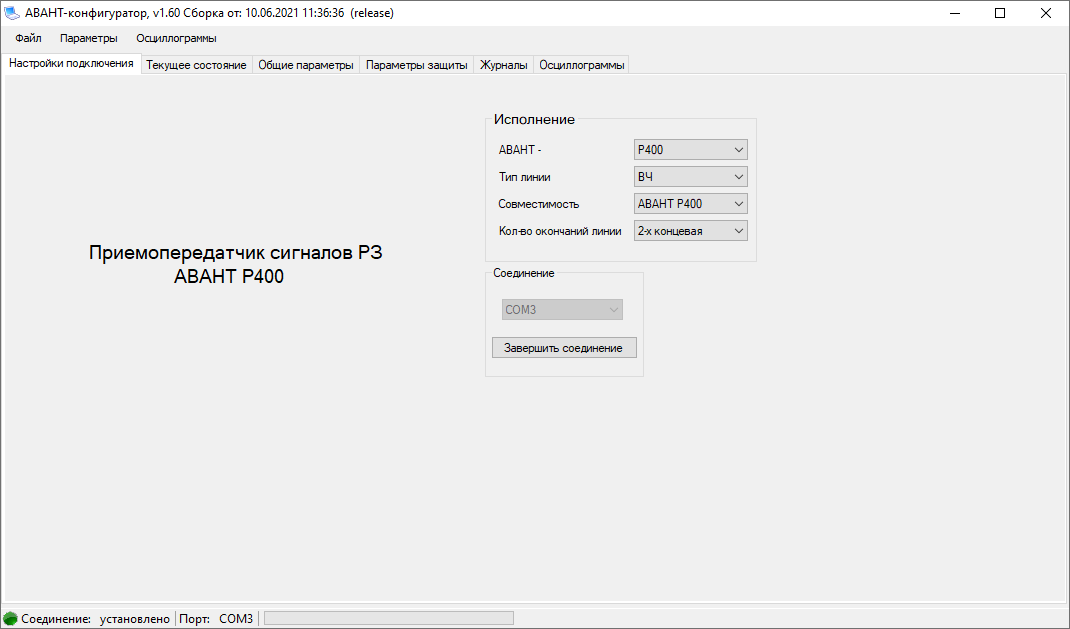
\includegraphics[width=0.8\linewidth]{configurator_connect.png}}
	
	\caption{Страница <<Настройки подключения>>}
	\label{fig:configurator_connect}
\end{figure}

Разорвать и вновь установить связь с приемопередатчиком возможно вручную с помощью кнопки <<Установить соединение>> на панели <<Соединение>> (рисунок \ref{fig:configurator_connect}), предварительно выбрав COM-порт, к которому подключен приемопередатчик. 

Вариант исполнения приемопередатчика представлен на панели <<Исполнение>>. 	
	
	
%%% ----------
\subsection{Страница <<Текущее состояние>>}	\label{ssec:configurator_state}

На данной странице (рисунок \ref{fig:configurator_state}) в режиме реального времени отображаются режим работы, текущее состояние, информация о наличии неисправностей приемопередатчика. Также на странице представлена информация об измеряемых параметрах.

\begin{figure}[H]
	\center{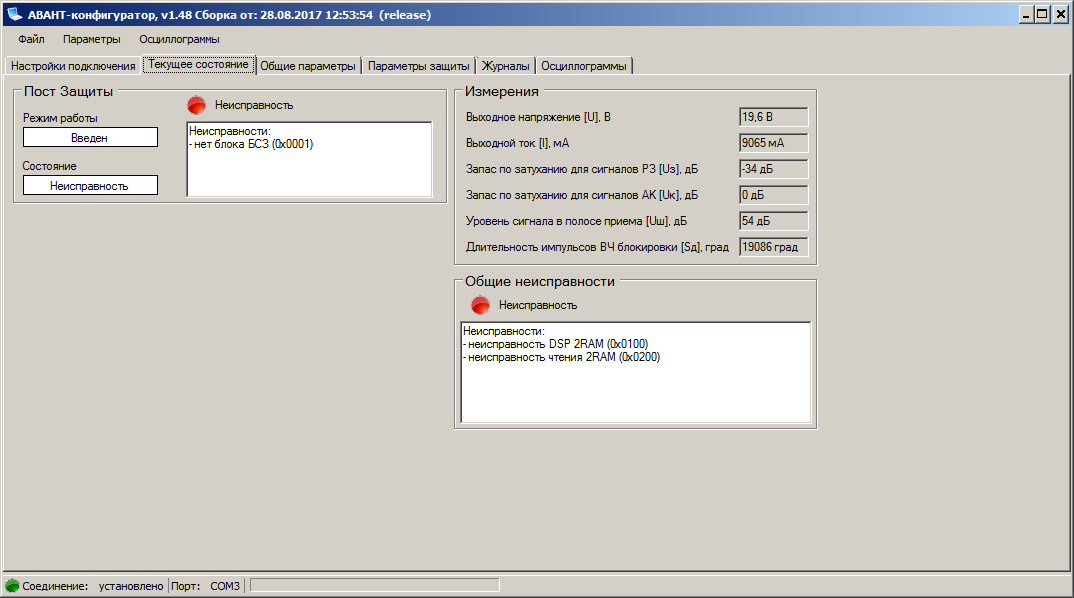
\includegraphics[width=0.8\linewidth]{configurator_state.png}}
	
	\caption{Страница <<Текущее состояние>>}
	\label{fig:configurator_state}
\end{figure}


%%% ----------
\subsection{Страница <<Общие параметры>>}	\label{ssec:configurator_param_glb}

На данной странице (рисунок \ref{fig:configurator_param_glb}) в режиме реального времени отображается режим работы приемопередатчика. На странице возможно изменение режима, изменение текущей даты и времени приемопередатчика, чтение, изменение и запись общих параметров работы приемопередатчика.

Запись параметров осуществляется только в режиме <<Выведен>>. 

\begin{figure}[H]
	\center{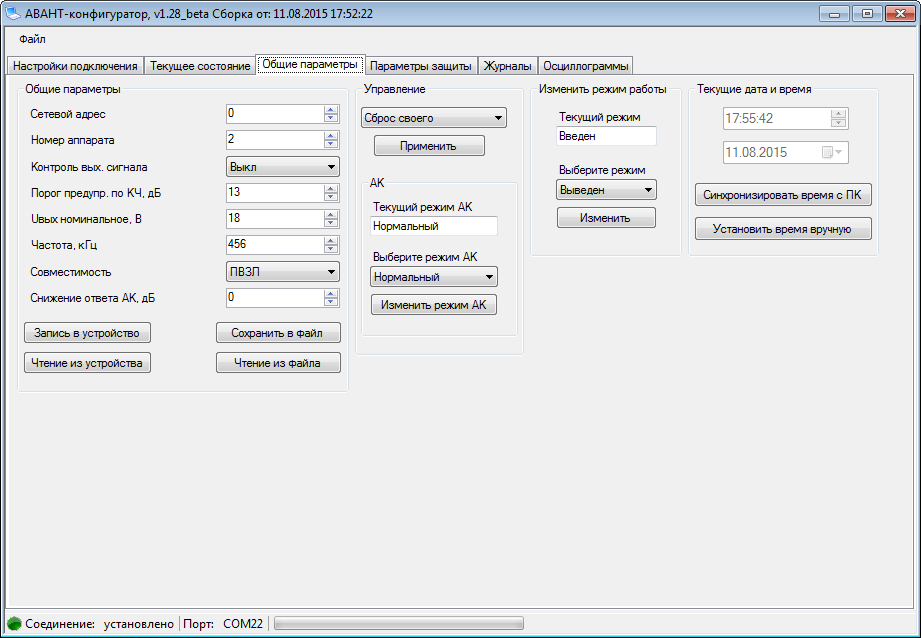
\includegraphics[width=0.8\linewidth]{configurator_param_glb.png}}
	
	\caption{Страница <<Общие параметры>>}
	\label{fig:configurator_param_glb}
\end{figure}

\textbf{Изменение режима}

Для изменения режима работы приемопередатчика необходимо на панели <<Изменить режим работы>> выбрать один из предложенных режимов и нажать на кнопку <<Изменить>>, после чего необходимо ввести пароль.
\newline

\textbf{Просмотр и изменение общих параметров}

Для того чтобы просмотреть установленные в настоящее время общие параметры работы приемопередатчика необходимо в верхней строке меню выбрать пункт <<Параметры>> $\rightarrow$ <<Чтение из устройства>> $\rightarrow$ <<Общие параметры>>. Считанные из приемопередатчика параметры отобразятся в соответствующих полях панели <<Общие параметры>>.

Для того чтобы изменить параметры необходимо ввести желаемые значения параметров и в верхней строке меню выбрать пункт <<Параметры>> $\rightarrow$ <<Запись в устройство>> $\rightarrow$ <<Общие параметры>>.
\newline

\textbf{В версиях приложения 1.53} и выше чтение и запись параметров осуществляется не раздельно по каждой группе (общие, защита), а всех сразу: в верхней строке меню пункт <<Параметры>> $\rightarrow$ <<Чтение всех параметров из устройства>> либо <<Параметры>> $\rightarrow$ <<Запись всех параметров в устройство>>.
\newline

\textbf{Сохранение и чтение общих параметров из файла}

Существует возможность сохранить измененные параметры работы приемопередатчика в файл, для этого необходимо в верхней строке меню выбрать пункт <<Параметры>> $\rightarrow$ <<Сохранить в файл>>, в появившемся окне выбрать место для сохранения, ввести имя файла и нажать <<Сохранить>>. В созданный файл будут сохранены все параметры работы приемопередатчика: общие параметры и параметры защиты.

Для того чтобы считать ранее сохраненные параметры из файла необходимо в верхней строке меню выбрать пункт <<Параметры>> $\rightarrow$ <<Загрузить из файла>>, в появившемся окне выбрать файл с параметрами и нажать <<Открыть>>. Из выбранного файла будут считаны все параметры работы приемопередатчика: общие параметры и параметры защиты. Для записи в приемопередатчик считанных из файла параметров необходимо в верхней строке меню выбрать пункт <<Параметры>> $\rightarrow$ <<Запись в устройство>> $\rightarrow$ <<Общие параметры>>. \textbf{В версиях приложения 1.53} и выше: <<Параметры>> $\rightarrow$ <<Запись всех параметров в устройство>>.
\newline

\textbf{Панель <<Управление>>}

С помощью панели <<Управление>> можно осуществить наладочный пуск передатчика сигналов защит на пять минут, запустить удаленный передатчик защиты на одну минуту, сбросить неисправности своего и удаленного приемопередатчика, включить вызывной сигнал на удаленном приемопередатчике (приглашение к переговорам), осуществить внеочередной запуск автоконтроля на своем и удаленном приемопередатчике, сбросить неисправности автоконтроля на своем и удаленном приемопередатчиках.
\newline

\textbf{Изменение значения даты и времени часов приемопередатчика}

Для изменения значения даты и времени часов приемопередатчика можно воспользоваться кнопкой <<Синхронизировать время с ПК>>, при этом дата и время в приемопередатчике установятся равными дате и времени подключенного ПК. Существует возможность установки часов вручную, для этого необходимо нажать на кнопку <<Установить время вручную>>, поля текущего времени и даты станут доступными для изменения, название кнопки изменится на <<Записать время в устройство>>. После чего необходимо ввести желаемые дату и время, нажать на кнопку <<Записать время в устройство>>. Название кнопки вновь изменится на <<Установить время вручную>>. 


%%% ----------
\subsection{Страница <<Параметры защиты>>}	\label{ssec:configurator_param_def}

На данной странице (рисунок \ref{fig:configurator_param_def}) возможны чтение, изменение и запись в приемопередатчик параметров защиты.

Запись параметров осуществляется только в режиме <<Выведен>>.

\begin{figure}[H]
	\center{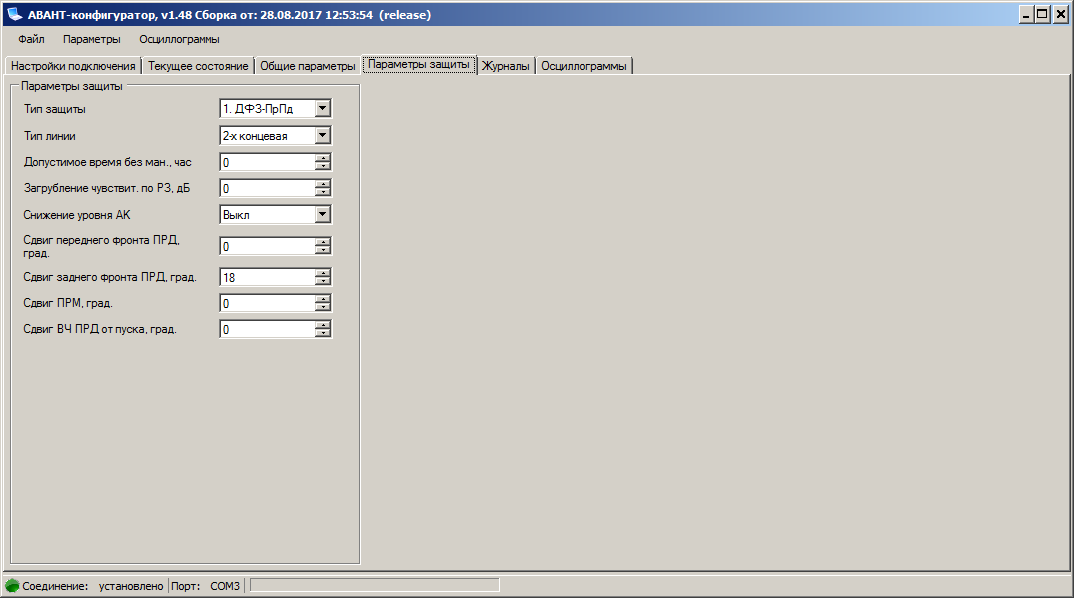
\includegraphics[width=0.8\linewidth]{configurator_param_def.png}}
	
	\caption{Страница <<Параметры защиты>>}
	\label{fig:configurator_param_def}
\end{figure}

\textbf{Просмотр и изменение параметров защиты}

Для того чтобы просмотреть установленные в настоящее время параметры работы приемопередатчика ВЧ защит необходимо в верхней строке меню выбрать пункт
<<Параметры>> $\rightarrow$ <<Чтение из устройства>> $\rightarrow$ <<Параметры защиты>>. Считанные из приемопередатчика параметры отобразятся в соответствующих полях панели <<Параметры защиты>>.

Для того чтобы изменить параметры необходимо ввести желаемые значения параметров и в верхней строке меню выбрать пункт <<Параметры>> $\rightarrow$ <<Запись в устройство>> $\rightarrow$ «Параметры защиты».

\textbf{В версиях приложения 1.53} и выше чтение и запись параметров осуществляется не раздельно по каждой группе (общие, защита), а всех сразу: в верхней строке меню пункт <<Параметры>> $\rightarrow$ <<Чтение всех параметров из устройства>> либо <<Параметры>> $\rightarrow$ <<Запись всех параметров в устройство>>. 
\newline 

\textbf{Сохранение и чтение параметров из файла}

Существует возможность сохранить измененные параметры работы приемопередатчика в файл, для этого необходимо в верхней строке меню выбрать пункт <<Параметры>> $\rightarrow$ <<Сохранить в файл>>, в появившемся окне выбрать место для сохранения, ввести имя файла и нажать <<Сохранить>>. В созданный файл будут сохранены все параметры работы приемопередатчика: общие параметры и параметры защиты.

Для того чтобы считать ранее сохраненные параметры из файла необходимо в верхней строке меню выбрать пункт <<Параметры>> $\rightarrow$ <<Загрузить из файла>>, в появившемся окне выбрать файл с параметрами и нажать <<Открыть>>. Из выбранного файла будут считаны все параметры работы приемопередатчика: общие параметры и параметры защиты. 

Для записи в приемопередатчик считанных из файла параметров необходимо в верхней строке меню выбрать пункт <<Параметры>> $\rightarrow$ <<Запись в устройство>> $\rightarrow$ <<Параметры защиты>>. \textbf{В версиях приложения 1.53} и выше: <<Параметры>> $\rightarrow$ <<Запись всех параметров в устройство>>.


%%% ----------
\subsection{Страница <<Журналы>>}	\label{ssec:configurator_journal}

В верхнем левом углу страницы <<Журналы>> (рисунок \ref{fig:configurator_journal_evt}) расположены закладки, соответствующие различным журналам:
\begin{enumerate}
	\item[1.] журнал событий – журнал общих событий и неисправностей приемопередатчика;
	\item[2.] журнал защиты – журнал работы приемопередатчика с терминалом защиты: запись управляющих воздействий от терминала (пуск передатчика, останов, манипуляция), запись фактов приема и передачи ВЧ сигналов.
\end{enumerate}

На каждой из страниц журналов расположены:
\begin{enumerate}
	\item[1.] кнопки управления: <<Чтение журнала>>, <<Сохранить в файл>>, <<Загрузить из файла>>;
	\item[2.] строка состояния, в которой отображается название журнала и количество записей в нем;
	\item[3.] таблица с записями журнала.
\end{enumerate}

\begin{figure}[H]
	\center{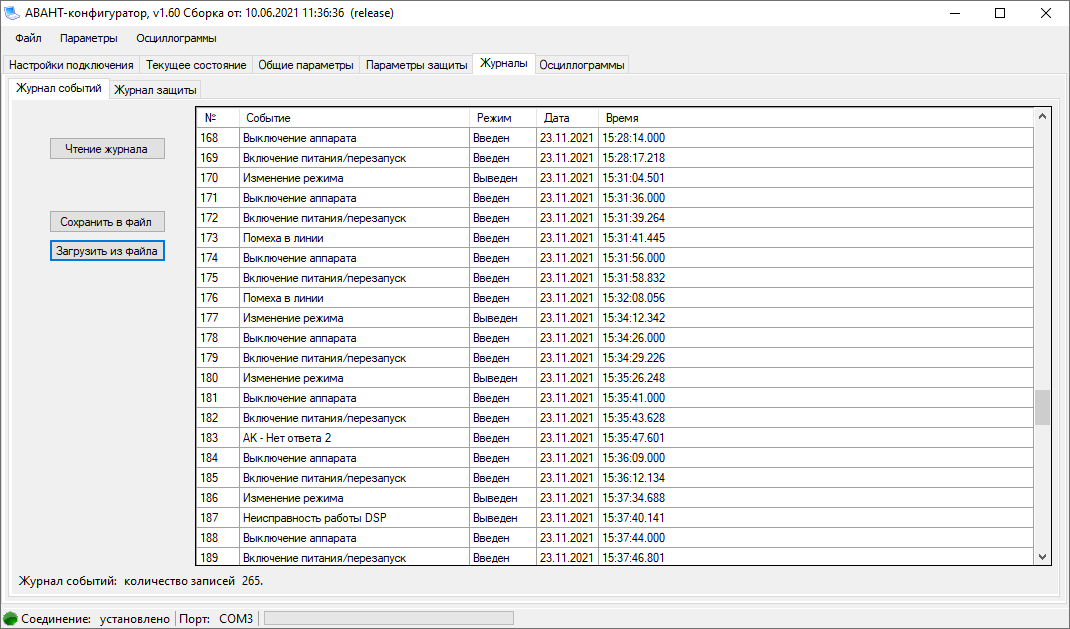
\includegraphics[width=0.9\linewidth]{configurator_journal_evt.png}}
	
	\caption{Страница <<Журналы: События>>}
	\label{fig:configurator_journal_evt}
\end{figure}

\textbf{Чтение журнала}

Для того чтобы считать журнал из приемопередатчика, необходимо нажать на кнопку <<Чтение журнала>>, при этом начнется чтение соответствующего журнала, внизу страницы в строке состояния отобразится количество записей данного журнала. После завершения чтения журнала все записи отобразятся в таблице.

Таблица журнала событий состоит из следующих колонок:
\begin{enumerate}
	\item[1.] № – номер записи;
	\item[2.] Событие – произошедшее событие, неисправность;
	\item[3.] Режим – режим работы приемопередатчика, при котором произошло событие;
	\item[4.] Дата события;
	\item[5.] Время события.
\end{enumerate}

Таблица журнала защиты состоит из следующих колонок:
\begin{enumerate}
	\item[1.] № – номер записи;
	\item[2.] Дата события;
	\item[3.] Время события.
	\item[4.] Состояние – состояние приемопередатчика, при котором произошло событие;
	\item[5.] Пуск – состояние входа <<Пуск>> на блоке КСЗ (<<0>> – в данный момент управляющего воздействия на вход нет; <<1>> – подано управляющее воздействие на вход).
	\item[6.] Останов – состояние входа <<Останов>> на блоке КСЗ (<<0>> – в данный момент управляющего воздействия на вход нет; <<1>> – подано управляющее воздействие на вход).
	\item[7.] МАН – состояние входа манипуляции на блоке КСЗ (<<0>> – в данный момент управляющего воздействия на вход нет; <<1>> – подано управляющее воздействие на вход).
	\item[8.] ПРД – состояние передатчика сигналов защит (<<0>> – передатчик остановлен, <<1>> –передатчик запущен).
	\item[9.] ПРМ – состояние приемника сигналов защит (<<0>> – приемник не принимает сигнал защиты, <<1>> – приемник принимает сигнал защиты).
	\item[10.] Выход приемника – состояние выхода приемника (<<0>> – в данный момент выход приемника не блокирован, <<1>> – выход приемника блокирован приемом сигнала защиты).
\end{enumerate}
	
В последней строке журнала выводятся дата и время считывания журнала из устройства. Дата и время считывания журнала берутся из устройства, а не из подключенного ПК.	
\newline		

\textbf{Сохранение и чтение журнала из файла}

Существует возможность сохранить каждый журнал в файл, для этого необходимо нажать на кнопку <<Сохранить в файл>>, в появившемся окне выбрать место для сохранения, ввести имя файла и нажать <<Сохранить>>. В созданный файл будет сохранен соответствующий журнал данных. 

Для того чтобы считать ранее сохраненный журнал из файла, необходимо нажать на кнопку <<Загрузить из файла>>, в появившемся окне выбрать файл с журналом и нажать <<Открыть>>. Из выбранного файла в таблицу конфигуратора будет загружен соответствующий журнал данных.


%%% ----------
\subsection{Страница <<Осциллограммы>>}	\label{ssec:configurator_oscillogram}

На данной странице (рисунок \ref{fig:configurator_oscillogram}) отображаются осциллограммы управляющих сигналов от панели защит – Пуск, Останов, Манипуляция; факты передачи и приема сигналов РЗ – ПРД, ПРМ; состояние выходной цепи приемника – Выход ПРМ.

Осциллограммы отображаются автоматически после чтения журнала защиты из приемопередатчика либо из ранее сохраненного файла с журналом защиты.

Управление осциллограммами производится с помощью мыши. Для того чтобы перемещать осциллограммы относительно меток времени, нужно нажать на правую кнопку
мыши и, удерживая ее, перемещать курсор вправо или влево.

Для того чтобы изменить масштаб осциллограммы по горизонтали, нужно нажать на левую кнопку мыши и, удерживая ее, переместить курсор вправо или влево. При этом
пунктирными линиями будет выделен отрезок времени, масштаб которого будет изменен. После чего отпустить левую кнопку мыши, выделенный отрезок времени будет растянут на все окно осциллограмм.

\begin{figure}[H]
	\center{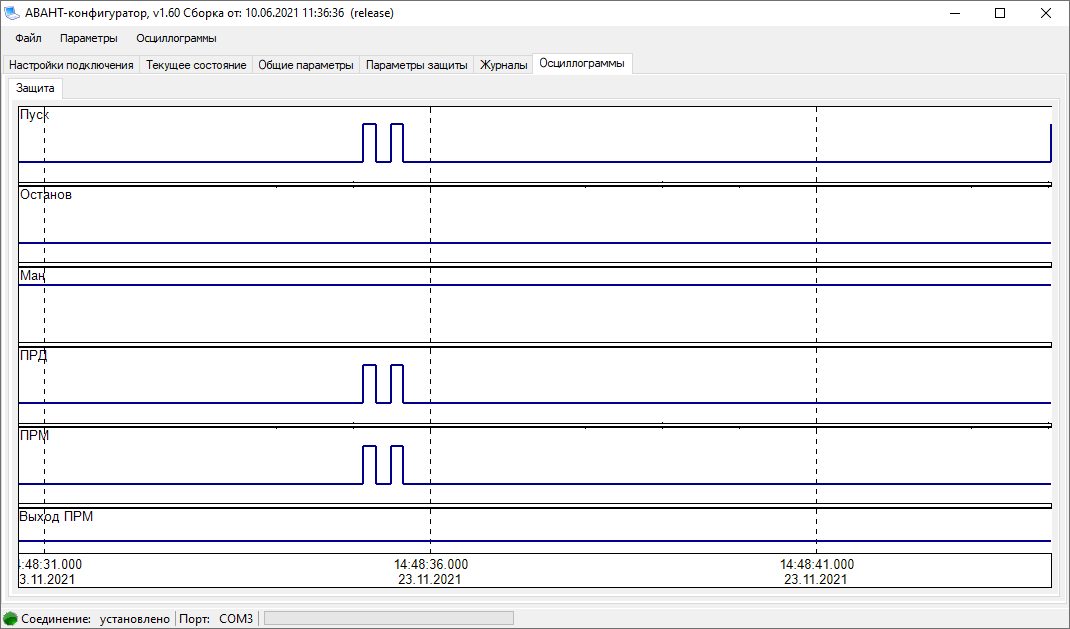
\includegraphics[width=0.9\linewidth]{configurator_oscillogram.png}}
	
	\caption{Страница <<Журналы: События>>}
	\label{fig:configurator_oscillogram}
\end{figure}

Изменять масштаб осциллограмм также возможно с помощью колеса мыши.

Для того чтобы вернуть масштаб осциллограммы в его начальное значение, необходимо в верхней строке меню выбрать пункт <<Осциллограммы>> $\rightarrow$ <<Установить масштаб по умолчанию>>.

Существует возможность сохранить осциллограммы в виде графического рисунка (файл с расширением «.jpg»), для этого необходимо в верхней строке меню выбрать пункт <<Осциллограммы>> $\rightarrow$ <<Сохранить как изображение>>, в появившемся окне выбрать место для сохранения, ввести имя файла и нажать кнопку <<Сохранить>>.

 	
 	%%% ----------
\ESKDappendix{Обязательное}{Неисправности и предупреждения} \label{app:err}

\begin{tabularx}{\linewidth}{| M{2cm} | m{4.5cm}| X |}
	\caption{Общие неисправности} 
	\label{tab:appError_glb_error}	
	\tabularnewline 
    
    \firsthline
    
    \centering Код & 
    \centering Показания индикатора &     
    \centering Описание неисправности 
    \tabularnewline \hline  
    \endfirsthead
    
    \multicolumn{3}{l}{Продолжение таблицы \ref{tab:appError_glb_error}} 
    \tabularnewline \hline 
    \centering Код & 
    \centering Показания индикатора &     
    \centering Описание неисправности 
    \tabularnewline \hline 
  	\endhead
    
    \multicolumn{3}{r}{продолжение следует\ldots} 
	\endfoot
	\endlastfoot
    
    0x0001 & Неиспр.чт.FLASH	& Неисправность при чтении данных из микросхемы FLASH-памяти на блоке БСП.	\tabularnewline \hline
    0x0002 & Неиспр.зап.FLASH	& Неисправность при записи данных в микросхему FLASH-памяти на блоке БСП. 	\tabularnewline \hline
    0x0004 & Неиспр.чт.PLIS		& Неисправность при чтении данных из микросхемы ПЛИС на блоке БСП.	\tabularnewline \hline
    0x0008 & Неиспр.зап.PLIS	& Неисправность при записи данных в микросхему ПЛСИ на блоке БСП.	\tabularnewline \hline
    0x0010 & Неиспр.зап.2RAM	& Неисправность при записи данных в микросхему двухпортового внешнего ОЗУ на блоке БСП	\tabularnewline \hline
    0x0020 & АК-нет ответа		& Удаленный приемопередатчик не отвечает на вызов автоконтроля. \tabularnewline \hline
    0x0040 & АК-Снижен.запаса	& Снижение запаса по затуханию. \tabularnewline \hline
    0x0080 & Помеха в линии		& При автоконтроле, при незапущенных своем и удаленном приемопередатчиках, обнаружен сигнал на выходе приемника - помеха в линии. \tabularnewline \hline
    0x0100 & Неиспр.DSP			& Неисправность цифрового сигнального процессора на блоке БСП. \tabularnewline \hline
    0x0200 & Неиспр.чт.2RAM		& Неисправность при чтении данных из микросхемы двухпортового внешнего ОЗУ на блоке БСП. \tabularnewline \hline
    0x0400 & Ток покоя			& Во время автоконтроля, при незапущенных своем и удаленном передатчиках, обнаружен сигнал на выходе приемника.	\tabularnewline \hline
    0x0800 & Низкое напр.вых.	& При запущенном передатчике, напряжение на выходе усилителя мощности снизилось в два раза по сравнению с напряжением, указанным в параметре <<Uвых номинальное>>.	\tabularnewline \hline
    0x1000 & Высокое напр.вых.	& При запущенно передатчике, напряжение на выходе усилителя мощности выросло в полтора раза по сравнению с напряжением, указанным в параметре <<Uвых номинальное>>.	\tabularnewline \hline
    0x2000 & Неиспр. МК УМ		& Неисправность микроконтроллера на измерительной плате в блоке усилителя мощности.	\tabularnewline \hline
    0x4000 & ВЧ тракт восст.	& Восстановление канала связи между приемопередатчиками, при установленном режиме <<АК односторонний>>. 	\tabularnewline 
    
    \lasthline
\end{tabularx} 

\begin{tabularx}{\linewidth}{| M{2cm} | m{4.5cm}| m{10cm}|}
	\caption{Общие предупреждения} 
	\label{tab:appError_glb_warning}	
	\tabularnewline 
    
    \firsthline
    
    \centering Код & 
    \centering Показания индикатора &     
    \centering Описание предупреждения 
    \tabularnewline \hline  
    \endfirsthead
    
    \multicolumn{3}{l}{Продолжение таблицы \ref{tab:appError_glb_error}} 
    \tabularnewline \hline 
    \centering Код & 
    \centering Показания индикатора &     
    \centering Описание предупреждения  
    \tabularnewline \hline 
  	\endhead
    
    \multicolumn{3}{r}{продолжение следует\ldots} 
	\endfoot
	\endlastfoot
    
     0x0001 & Установите часы	& Сбой часов приемопередатчика.	\tabularnewline 
     
    \lasthline
\end{tabularx} 

\begin{tabularx}{\linewidth}{| M{2cm} | m{4.5cm}| X|}
	\caption{Неисправности защиты}  	
	\label{tab:appError_def_error}	\tabularnewline
    
     \firsthline
    
    \centering Код & 
    \centering Показания индикатора &     
    \centering Описание неисправности 
    \tabularnewline \hline  
    \endfirsthead
    
    \multicolumn{3}{l}{Продолжение таблицы \ref{tab:appError_def_error}} 
    \tabularnewline \hline 
    \centering Код & 
    \centering Показания индикатора &     
    \centering Описание неисправности 
    \tabularnewline \hline 
  	\endhead
    
    \multicolumn{3}{r}{продолжение следует\ldots} 
	\endfoot
	\endlastfoot
    
    0x0001 & Нет блока БСЗ		& Блок БСЗ отсутствует в каркасе с блоками, либо неисправнен. \tabularnewline \hline
    0x0002 & Неиспр.верс.БСЗ	& Версия блока БСЗ не соответствует текущей версии приемопередатчика, либо блок БСЗ неисправен. \tabularnewline \hline
    0x0004 & Неиспр.перекл.		& Положение переключателей S1.1 \ldots S1.4 на блоке БСЗ не соответсвует значению параметра <<Тип защиты>>. 	\tabularnewline \hline
    0x0008 & Неиспр.зап.БСЗ		& Ошибка записи в блок БСЗ.							\tabularnewline \hline
    0x0010 & АК-Нет ответа N	& Удаленный приемопередатчик не отвечает на вызов автоконтроля. N - номер не ответившего приемопередатчика. \tabularnewline \hline
    0x0020 & Низкий ур. РЗ		& \tabularnewline \hline
    0x0040 & Неиспр.уд.ДФЗ N	& Удаленный приемопередатчик обнаружил неисправность в тесте ДФЗ при автоконтроле. N - номер приемопередатчика обнаружившего неисправность. \tabularnewline \hline
    0x0080 & неиспр.уд.ВЫХ N	& Удаленный приемопередатчик обнаружил неисправность выходной цепи приемника. N - номер приемопередатчика обнаружившего неисправность. \tabularnewline \hline
    0x0100 & Неиспр.вход.ПУСК	& Неисправна входная цепь сигнала <<Пуск>>.			\tabularnewline \hline
    0x0200 & Неиспр.вход.СТОП	& Неисправна входная цепь сигнала <<СТОП>>.			\tabularnewline \hline
    0x0400 & Удал.без отв. N	& Удаленный приемопередатчик не получил ответ при автоконтроле. N - номер приемопередатчика обнаружившего неисправность.\tabularnewline \hline
    0x0800 & Неиспр.цепь ВЫХ	& Неисправность выходной цепи приемника:<<ПРМ~2>> либо <<РЗ вых>>. \tabularnewline \hline
    0x1000 & Удал.обн.пом. N	& Удаленный приемопередатчик обнаружил помеху при автоконтроле. N - номер приемопередатчика обнаружившего неисправность. \tabularnewline \hline
    0x2000 & Неиспр.зап.ВЫХ		& Неисправность выходной цепи приемника:<<ПРМ~2>> либо <<РЗ вых>>. \tabularnewline \hline
    0x4000 & Помеха в линии		& Во время автоконтроля, при незапущенных своем и удаленном передатчиках обнаружен сигнал на выходе приемника - помеха в линии. \tabularnewline \hline
    0x8000 & Неиспр. ДФЗ N		& Во время автоконтроля, в тесте ДФЗ обнаружена неисправность. N - номер приемопередатчика обнаружившего неисправность. \tabularnewline 
    
    \lasthline
\end{tabularx} 


\begin{tabularx}{\linewidth}{| M{2cm} | m{4.5cm}| X|}
	\caption{Предупреждения защиты}  	
	\label{tab:appError_def_warning}	\tabularnewline
    
     \firsthline
    
    \centering Код & 
    \centering Показания индикатора &     
    \centering Описание предупреждения
    \tabularnewline \hline  
    \endfirsthead
    
    \multicolumn{3}{l}{Продолжение таблицы \ref{tab:appError_def_warning}} 
    \tabularnewline \hline 
    \centering Код & 
    \centering Показания индикатора &     
    \centering Описание предупреждения 
    \tabularnewline \hline 
  	\endhead
    
    \multicolumn{3}{r}{продолжение следует\ldots} 
	\endfoot
	\endlastfoot
    
    0x0001 & АК-Сн.запаса N		& Снижение запаса по затуханию. N - номер приемопередатчика, со стороны которого увеличилось затухание. \tabularnewline \hline
    0x0002 & Нет сигнала МАН	& На входах <<Ман1>> или <<Ман2>> отсутствует напряжение манипуляции в течение времени, установленного в параметре <<Допустимое время без МАН>>. \tabularnewline \hline
    0x0004 & Порог по помехе	& По выходу приемника были накоплены импульсы помехи, суммарная длительность которых превысила значение параметра <<Порог по помехе>>. \tabularnewline \hline
    0x0008 & Автоконтроль		& В совместимости с ПВЗЛ: зафиксирован пропуск очередного автоматического пуска автоконтроля на противоположном конце линии. \newline В совместимости с ПВЗ-90: зафиксировано 12 вызовов автоконтроля от удаленного приемопередатчика, при этом свой приемопередатчика автоконтроль не проводил. \tabularnewline
    
    \lasthline
\end{tabularx}  	
 	%%% ----------
\ESKDappendix{Обязательное}{Расшифровка сообщений в журнале событий} \label{app:journal}

\begin{tabularx}{\linewidth}{| M{1cm} | m{3.5cm}| X |}
	\caption{Записи журнала событий} 
	\label{tab:appJournal}	
	\tabularnewline 
    
    \firsthline
    
    \centering № & 
    \centering Событие &     
    \centering Описание 
    \tabularnewline \hline  
    \endfirsthead
    
    \multicolumn{3}{l}{Продолжение таблицы \ref{tab:appJournal}} 
    \tabularnewline \hline 
    \centering № & 
    \centering Событие &     
    \centering Описание
    \tabularnewline \hline 
  	\endhead
    
    \multicolumn{3}{r}{продолжение следует\ldots} 
	\endfoot
	\endlastfoot
    
    1 	& Неис.FLASH	& Неисправность микросхемы памяти FLASH на блоке БСП.	\tabularnewline \hline
    2 	& ВЧ восст.		& Восстановление канала связи между приемопередатчиками, при этом установлен режим <<АК односторонний>>.	\tabularnewline \hline
    3 	& Неисп.PLIS	& Неисправность микросхемы ПЛИС на блоке БСП.	\tabularnewline \hline
    4 	& Автоконтр.	& В совместимости с ПВЗЛ: зафиксирован пропуск очередного автоматического пуска автоконтроля на противоположном конце линии. \newline В совместимости с ПВЗ-90: зафиксировано 12 вызовов автоконтроля от удаленного приемопередатчика, при этом свой приемопередатчик автоконтроль не проводил.	\tabularnewline \hline
    5 	& Ток покоя 	& Во время автоконтроля, при незапущенных своем и удаленном приемопередатчиках обнаружен сигнал на выходе приемника. \tabularnewline \hline
    6 	& Неисп.2RAM	& Неисправность микросхемы двухпортового внешнего ОЗУ на блоке БСП.	\tabularnewline \hline
    7 	& Н.раб.DSP		& Неисправность цифрового сигнального процессора на блоке БСП. 	\tabularnewline \hline
    8 	& Вост.р.DSP	& Восстановление нормальной работы цифрового сигнального процессора на блоке БСП.	\tabularnewline \hline
    9 	& Низк. Uвых	& При запущенном передатчике, напряжение на выходе усилителя мощности снизилось в два раза по сравнению с напряжением, указанных в параметре <<Uвых номинальное>>.	\tabularnewline \hline
	10 	& Выс. Uвых		& При запущенном передатчике, напряжение на выходе усилителя мощности выросло в полтора раза по сравнению с напряжением, указанным в параметре <<Uвых номинальное>>.	\tabularnewline \hline
	11	& Н.св. с УМ	& Неисправность микроконтроллера на измерительной плате в блоке усилителя мощности.	\tabularnewline \hline
	12	& Неис.часов	& Сбой часов приемопередатчика.	\tabularnewline \hline
	13	& Нет бл.БСЗ	& Блок БСЗ отсутствует в каркасе с блоками, либо неисправен.	\tabularnewline \hline
	14	& Н.верс.БСЗ	& Версия блока БСЗ не соответсвтует текущей версии приемопередатчика, либо блок БСЗ неисправен.	\tabularnewline \hline
	15	& Н.пер. БСЗ	& Положение переключателей S1.1 \ldots S1.4 на блоке БСЗ не соотвествует значению параметра <<Тип защиты>>.	\tabularnewline \hline
	16	& Нет с. МАН	& На входах <<Ман1>> или <<Ман2>> отсутствует напряжение манипуляции в течении времени установленного в параметре <<Допустимое время без МАН>>.	\tabularnewline \hline
	17	& Перезапуск	& Включение электропитания приемопередатчика.	\tabularnewline \hline
	18	& Изм.режима	& Изменение режима работы приемопередатчика.	\tabularnewline \hline
	19	& Н.цепи ВЫХ	& Неисправность выходной цепи приемника: <<ПРМ~2>> либо <<РЗ~вых>>	\tabularnewline \hline
	20	& Изм. парам	& Изменение параметров приемопередатчика.	\tabularnewline \hline
	21	& АК-сн.зап.	& Снижение запаса по затуханию.	\tabularnewline \hline
	22	& АК-нет отв	& Удаленный приемопередатчик не отвечает на вызов автоконтроля.	\tabularnewline \hline
	23	& Нет с.ПУСК	& Неисправность входной цепи <<Пуск>>.	\tabularnewline \hline
	24	& Нет с.СТОП	& Неисправность	входной цепи <<Стоп>>.\tabularnewline \hline
	25	& Выключение	& Выключение электропитания приемопередатчика.	\tabularnewline \hline
	26	& Помеха 		& При автоконтроле, при незапущенных своем и удаленном передатчиках, обнаружен сигнал на входе приемника. \newline В ПВЗ - помеха в канале связи. 	\tabularnewline \hline
	27	& Неиспр.ДФЗ	& Во время автоконтроля, в тесте ДФЗ обнаружена неисправность.	\tabularnewline \hline
	28	& Уд: Нет АК	& Удаленный приемопередатчик не получил ответа при автоконтроле.	\tabularnewline \hline
	29	& Уд: Помеха	& Удаленный приемопередатчик обнаружил помеху при автоконтроле.	\tabularnewline \hline
	30	& Уд: Н. ДФЗ	& Удаленный приемопередатчик обнаружил неисправность в тесте ДФЗ при автоконтроле.	\tabularnewline \hline
	31	& Уд: Н. ВЫХ	& Удаленный приемопередатчик обнаружил неисправность выходной цепи приемника.	\tabularnewline \hline
	32 	& Пор.помех		& По выходу приемника были накоплены импульсы помехи, суммарная длительность которых превысила значение параметра <<Порог по помехе>>.	\tabularnewline \hline
	33 	& Изм. время	& \tabularnewline \hline
	34 	& Часы 			& Неисправность часов приемопередатчика.	\tabularnewline \hline
	35  & Помеха        & \tabularnewline \hline
	36 	& Дальний		& Неисправность приемопередатчика противоположного конца канала связи.	\tabularnewline \hline
	37  & Сбр.своего    & \tabularnewline \hline
	38  & Сбр.от уд.    & \tabularnewline \hline
	39  & Сброс АК      & \tabularnewline \hline
	40  & Сбр.АК упр    & \tabularnewline \hline
	41  & Сбр АК уд.    & \tabularnewline \hline
	42  & Пуск АК       & \tabularnewline
		
	\lasthline
\end{tabularx} 
	%%% ----------
\ESKDappendix{Обязательное}{Управление} \label{app:control}

\begin{tabularx}{\linewidth}{| M{0.6cm} | m{4.9cm} | m{11.2cm} |}
	\caption{Команды управления в совместимости Р400 }  	 
	\label{tab:appСontrol_p400}	\tabularnewline
    
    \firsthline
    
    \centering № п/п &
    \centering Показания индикатора &
    \centering Измеряемый параметр
    \tabularnewline \hline
    \endfirsthead

    \multicolumn{3}{l}{Продолжение таблицы~\ref{tab:appControl_p400}}
    \tabularnewline \hline
    \centering № п/п &
    \centering Показания индикатора &
    \centering Измеряемый параметр
    \tabularnewline \hline
  	\endhead

    \multicolumn{3}{r}{продолжение следует\ldots}
	\endfoot
	\endlastfoot
    
    \multicolumn{3}{|c|}{2-х концевая линия} \tabularnewline \hline
    0	& Пуск налад.вкл. \newline Пуск налад.выкл.	& Наладочный пуск передатчика: включение/выключение передатчика на пять минут. \tabularnewline \hline
    1	& Сброс своего. 		& Сброс неисправностей приемопередатчика.	 			\tabularnewline \hline
    2	& Сброс  удаленного. 	& Сброс неисправностей на удаленном приемопередатчике. 	\tabularnewline \hline
    3	& Пуск удаленного.		& Пуск удаленного передатчика на 20 с.  				\tabularnewline \hline
    4	& Вызов.				& Включение вызывного сигнала на удаленном приемопередатчике (приглашение к переговорам). \tabularnewline \hline

    \multicolumn{3}{|c|}{3-х концевая линия} \tabularnewline \hline
    0	& Пуск налад.вкл. \newline Пуск налад.выкл.	& Наладочный пуск передатчика: включение/выключение передатчика на пять минут. \tabularnewline \hline
    1	& Сброс своего. 		& Сброс неисправностей приемопередатчика.	 				\tabularnewline \hline
    2	& Сброс удаленного X. 	& Сброс неисправностей на удаленном приемопередатчике X. 	\tabularnewline \hline
    3	& Сброс удаленного Y. 	& Сброс неисправностей на удаленном приемопередатчике Y. 	\tabularnewline \hline
    4	& Пуск удаленного X.	& Пуск удаленного передатчика X на 20~с.  					\tabularnewline \hline
    5	& Пуск удаленного Y.	& Пуск удаленного передатчика Y на 20~с.  					\tabularnewline \hline
    6	& Пуск удаленных.		& Пуск всех удаленных передатчиков на 20~c.  				\tabularnewline \hline
    7	& Вызов.				& Включение вызывного сигнала на удаленном приемопередатчике (приглашение к переговорам). \tabularnewline
  
    \lasthline
\end{tabularx} 


\begin{tabularx}{\linewidth}{| M{0.6cm} | m{4.9cm} | m{11.2cm} |}
	\caption{Команды управления в совместимости ПВЗ-90}  	 
	\label{tab:appControl_pvz90}	\tabularnewline
    
    \firsthline
    
    \centering № п/п & 
    \centering Показания индикатора &     
    \centering Измеряемый параметр
    \tabularnewline \hline  
    \endfirsthead
    
    \multicolumn{3}{l}{Продолжение таблицы~\ref{tab:appControl_pvz90}} 
    \tabularnewline \hline 
    \centering № п/п & 
    \centering Показания индикатора &     
    \centering Измеряемый параметр
    \tabularnewline \hline 
  	\endhead
    
    \multicolumn{3}{r}{продолжение следует\ldots} 
	\endfoot
	\endlastfoot
    
    0	& Пуск налад.вкл. \newline Пуск налад.выкл.	& Наладочный пуск передатчика: включение/выключение передатчика на пять минут. \tabularnewline \hline
    1	& Сброс своего. 		& Сброс неисправностей приемопередатчика.	 			\tabularnewline \hline
    2	& Сброс  удаленного. 	& Сброс неисправностей на удаленном приемопередатчике. 	\tabularnewline \hline
	% TODO в Р400м и конфигураторе сигнала Вызов нет
    3	& Вызов.				& Включение вызывного сигнала на удаленном приемопередатчике (приглашение к переговорам). \tabularnewline
  
    \lasthline
\end{tabularx}


\begin{tabularx}{\linewidth}{| M{0.6cm} | m{4.9cm} | m{11.2cm} |}
	\caption{Команды управления в совместимости АВЗК-80}  	 
	\label{tab:appControl_avzk80}	\tabularnewline
    
    \firsthline
    
    \centering № п/п & 
    \centering Показания индикатора &     
    \centering Измеряемый параметр
    \tabularnewline \hline  
    \endfirsthead
    
    \multicolumn{3}{l}{Продолжение таблицы~\ref{tab:appControl_avzk80}} 
    \tabularnewline \hline 
    \centering № п/п & 
    \centering Показания индикатора &     
    \centering Измеряемый параметр
    \tabularnewline \hline 
  	\endhead
    
    \multicolumn{3}{r}{продолжение следует\ldots} 
	\endfoot
	\endlastfoot
    
    0	& Пуск налад.вкл. \newline Пуск налад.выкл.	& Наладочный пуск передатчика: включение/выключение передатчика на пять минут. \tabularnewline \hline
    1	& Сброс своего. 		& Сброс неисправностей приемопередатчика.	 			\tabularnewline \hline
	% TODO в Р400м и конфигураторе сигнала Вызов нет
    2	& Вызов.				& Включение вызывного сигнала на удаленном приемопередатчике (приглашение к переговорам). \tabularnewline
  
    \lasthline
\end{tabularx}


\begin{tabularx}{\linewidth}{| M{0.6cm} | m{4.9cm} | m{11.2cm} |}
	\caption{Команды управления в совместимости ПВЗУ-Е }  	 
	\label{tab:appControl_pvzue}	\tabularnewline
    
    \firsthline
    
    \centering № п/п & 
    \centering Показания индикатора &     
    \centering Измеряемый параметр
    \tabularnewline \hline  
    \endfirsthead
    
    \multicolumn{3}{l}{Продолжение таблицы~\ref{tab:appControl_pvzue}}
    \tabularnewline \hline 
    \centering № п/п & 
    \centering Показания индикатора &     
    \centering Измеряемый параметр
    \tabularnewline \hline 
  	\endhead
    
    \multicolumn{3}{r}{продолжение следует\ldots} 
	\endfoot
	\endlastfoot
    
    \multicolumn{3}{|c|}{2-х концевая линия} \tabularnewline \hline
    0	& Пуск налад.вкл. \newline Пуск налад.выкл.	& Наладочный пуск передатчика: включение/выключение передатчика на пять минут. \tabularnewline \hline
    1	& Сброс своего. 		& Сброс неисправностей приемопередатчика.	 			\tabularnewline \hline
    2 	& Пуск удаленного.		& Пуск удаленного передатчика на 15 с.  				\tabularnewline \hline 
    3 	& Пуск удален. МАН		& Пуск удаленного передатчика манипулированным сигналом на 15 с.		\tabularnewline \hline 
    4 	& Пуск удал-ых. МАН		& Пуск всех удаленных передатчиков манипулированным сигна-лом на 15 с.	\tabularnewline \hline 
    5	& Вызов.				& Включение вызывного сигнала на удаленном приемопередатчике (приглашение к переговорам). \tabularnewline \hline
    
    \multicolumn{3}{|c|}{3-х концевая линия} \tabularnewline \hline
    0	& Пуск налад.вкл. \newline Пуск налад.выкл.	& Наладочный пуск передатчика: включение/выключение передатчика на пять минут. \tabularnewline \hline
    1	& Сброс своего. 		& Сброс неисправностей приемопередатчика.	 				\tabularnewline \hline
    2	& Сброс  удаленного X. 	& Сброс неисправностей на удаленном приемопередатчике X. 	\tabularnewline \hline
    3	& Сброс  удаленного Y. 	& Сброс неисправностей на удаленном приемопередатчике Y. 	\tabularnewline \hline
    4	& Пуск удал. МАН X.		& Пуск удаленного передатчика X манипулированным сигналом на 15 с.  	\tabularnewline \hline
    5	& Пуск удал. МАН Y.		& Пуск удаленного передатчика Y манипулированным сигналом на 15 с.  	\tabularnewline \hline
    6 	& Пуск удал-ых. МАН		& Пуск всех удаленных передатчиков манипулированным сигна-лом на 15 с.	\tabularnewline \hline 
    7	& Вызов.				& Включение вызывного сигнала на удаленном приемопередатчике (приглашение к переговорам). \tabularnewline \hline
    
    \multicolumn{3}{|c|}{4-х концевая (и более) линия} \tabularnewline \hline
    0	& Пуск налад.вкл. \newline Пуск налад.выкл.	& Наладочный пуск передатчика: включение/выключение передатчика на пять минут. \tabularnewline \hline
    1	& Сброс своего. 		& Сброс неисправностей приемопередатчика.	 				\tabularnewline \hline
    2	& Сброс  удаленного X. 	& Сброс неисправностей на удаленном приемопередатчике X. 	\tabularnewline \hline
    3	& Сброс  удаленного Y. 	& Сброс неисправностей на удаленном приемопередатчике Y. 	\tabularnewline \hline
    4	& Сброс  удаленного Z. 	& Сброс неисправностей на удаленном приемопередатчике Z. 	\tabularnewline \hline
    5	& Пуск удал. МАН X.		& Пуск удаленного передатчика X манипулированным сигналом на 15 с.  	\tabularnewline \hline
    6	& Пуск удал. МАН Y.		& Пуск удаленного передатчика Y манипулированным сигналом на 15 с.  	\tabularnewline \hline
    7	& Пуск удал. МАН Z.		& Пуск удаленного передатчика Z манипулированным сигналом на 15 с.  	\tabularnewline \hline
    8 	& Пуск удал-ых. МАН		& Пуск всех удаленных передатчиков манипулированным сигна-лом на 15 с.	\tabularnewline \hline 
    9	& Вызов.				& Включение вызывного сигнала на удаленном приемопередатчике (приглашение к переговорам). \tabularnewline
  
    \lasthline
\end{tabularx}


\begin{tabularx}{\linewidth}{| M{0.6cm} | m{4.9cm} | m{11.2cm} |}
	\caption{Команды управления в совместимости ПВЗЛ}  	 
	\label{tab:appControl_pvzl}	\tabularnewline
    
    \firsthline
    
    \centering № п/п & 
    \centering Показания индикатора &     
    \centering Измеряемый параметр
    \tabularnewline \hline  
    \endfirsthead
    
    \multicolumn{3}{l}{Продолжение таблицы~\ref{tab:appControl_pvzl}} 
    \tabularnewline \hline 
    \centering № п/п & 
    \centering Показания индикатора &     
    \centering Измеряемый параметр
    \tabularnewline \hline 
  	\endhead
    
    \multicolumn{3}{r}{продолжение следует\ldots} 
	\endfoot
	\endlastfoot
    
    0	& Пуск налад.вкл. \newline Пуск налад.выкл.	& Наладочный пуск передатчика: включение/выключение передатчика на пять минут. \tabularnewline \hline
    1	& Сброс своего. 		& Сброс неисправностей приемопередатчика.	 						\tabularnewline \hline
    2	& Пуск АК удаленный 	& Внеочередной запуск автоконтроля на удаленном приемопередатчике. 	\tabularnewline \hline
    3 	& Пуск ПРД				& Пуск удаленного передатчика на 10 секунд.							\tabularnewline \hline
    4	& Вызов.				& Включение вызывного сигнала на удаленном приемопередатчике (приглашение к переговорам). \tabularnewline
  
    \lasthline
\end{tabularx}


\begin{tabularx}{\linewidth}{| M{0.6cm} | m{4.9cm} | m{11.2cm} |}
	\caption{Команды управления в совместимости Линия-Р }  	 
	\label{tab:appControl_liner}	\tabularnewline
    
    \firsthline
    
    \centering № п/п &
    \centering Показания индикатора &
    \centering Измеряемый параметр
    \tabularnewline \hline
    \endfirsthead

    \multicolumn{3}{l}{Продолжение таблицы~\ref{tab:appControl_liner}}
    \tabularnewline \hline
    \centering № п/п &
    \centering Показания индикатора &
    \centering Измеряемый параметр
    \tabularnewline \hline
  	\endhead

    \multicolumn{3}{r}{продолжение следует\ldots}
	\endfoot
	\endlastfoot

    \multicolumn{3}{|c|}{2-х концевая линия} \tabularnewline \hline
    0	& Пуск налад.вкл. \newline Пуск налад.выкл.	& Наладочный пуск передатчика: включение/выключение передатчика на пять минут. \tabularnewline \hline
    1	& Сброс своего. 		& Сброс неисправностей приемопередатчика.	 			\tabularnewline \hline
    2	& Сброс  удаленного. 	& Сброс неисправностей на удаленном приемопередатчике. 	\tabularnewline \hline
    3	& Пуск удаленного.		& Пуск удаленного передатчика на 20 с.  				\tabularnewline \hline
    4	& Вызов.				& Включение вызывного сигнала на удаленном приемопередатчике (приглашение к переговорам). \tabularnewline \hline

    \multicolumn{3}{|c|}{3-х концевая линия} \tabularnewline \hline
    0	& Пуск налад.вкл. \newline Пуск налад.выкл.	& Наладочный пуск передатчика: включение/выключение передатчика на пять минут. \tabularnewline \hline
    1	& Сброс своего. 		& Сброс неисправностей приемопередатчика.	 				\tabularnewline \hline
    2	& Сброс удаленного X. 	& Сброс неисправностей на удаленном приемопередатчике X. 	\tabularnewline \hline
    3	& Сброс удаленного Y. 	& Сброс неисправностей на удаленном приемопередатчике Y. 	\tabularnewline \hline
    4	& Пуск удаленного X.	& Пуск удаленного передатчика X на 20~с.  					\tabularnewline \hline
    5	& Пуск удаленного Y.	& Пуск удаленного передатчика Y на 20~с.  					\tabularnewline \hline
    6	& Пуск удаленных.		& Пуск всех удаленных передатчиков на 20~c.  				\tabularnewline \hline
    7	& Вызов.				& Включение вызывного сигнала на удаленном приемопередатчике (приглашение к переговорам). \tabularnewline
  
    \lasthline
\end{tabularx} 


\begin{tabularx}{\linewidth}{| M{0.6cm} | m{4.9cm} | m{11.2cm} |}
	\caption{Команды управления в совместимости ПЗВК }  	 
	\label{tab:appControl_pvzk}	\tabularnewline
    
    \firsthline
    
    \centering № п/п &
    \centering Показания индикатора &
    \centering Измеряемый параметр
    \tabularnewline \hline
    \endfirsthead

    \multicolumn{3}{l}{Продолжение таблицы~\ref{tab:appControl_pvzk}}
    \tabularnewline \hline
    \centering № п/п & 
    \centering Показания индикатора &     
    \centering Измеряемый параметр
    \tabularnewline \hline 
  	\endhead

    \multicolumn{3}{r}{продолжение следует\ldots}
	\endfoot
	\endlastfoot
    
    0	& Пуск налад.вкл. \newline Пуск налад.выкл.	& Наладочный пуск передатчика: включение/выключение передатчика на пять минут. \tabularnewline \hline
    1	& Сброс своего. 		& Сброс неисправностей приемопередатчика.	 			\tabularnewline \hline
    % TODO в конфигураторе только сигнал Сброс своего
    2	& Сброс  удаленного. 	& Сброс неисправностей на удаленном приемопередатчике. 	\tabularnewline \hline
    3	& Пуск удаленного.		& Пуск удаленного передатчика на 20 с.  				\tabularnewline \hline
    4	& Вызов.				& Включение вызывного сигнала на удаленном приемопередатчике (приглашение к переговорам). \tabularnewline 
  
    \lasthline
\end{tabularx} 


\begin{tabularx}{\linewidth}{| M{0.6cm} | m{4.9cm} | m{11.2cm} |}
	\caption{Команды управления в совместимости ПВЗУ}  	 
	\label{tab:appControl_pvzu}	\tabularnewline
    
    \firsthline
    
    \centering № п/п & 
    \centering Показания индикатора &     
    \centering Измеряемый параметр
    \tabularnewline \hline  
    \endfirsthead
    
    \multicolumn{3}{l}{Продолжение таблицы~\ref{tab:appControl_pvzu}} 
    \tabularnewline \hline 
    \centering № п/п & 
    \centering Показания индикатора &     
    \centering Измеряемый параметр
    \tabularnewline \hline 
  	\endhead
    
    \multicolumn{3}{r}{продолжение следует\ldots} 
	\endfoot
	\endlastfoot
    
    0	& Пуск налад.вкл. \newline Пуск налад.выкл.	& Наладочный пуск передатчика: включение/выключение передатчика на пять минут. \tabularnewline \hline
    1	& Сброс своего. 		& Сброс неисправностей приемопередатчика.	 			\tabularnewline \hline
    2	& Вызов.				& Включение вызывного сигнала на удаленном приемопередатчике (приглашение к переговорам). \tabularnewline
  
    \lasthline
\end{tabularx}


\begin{tabularx}{\linewidth}{| M{0.6cm} | m{4.9cm} | m{11.2cm} |}
	\caption{Команды управления в совместимости ПВЗ}  	 
	\label{tab:appControl_pvz}	\tabularnewline
    
    \firsthline
    
    \centering № п/п & 
    \centering Показания индикатора &     
    \centering Измеряемый параметр
    \tabularnewline \hline  
    \endfirsthead
    
    \multicolumn{3}{l}{Продолжение таблицы~\ref{tab:appControl_pvz}} 
    \tabularnewline \hline 
    \centering № п/п & 
    \centering Показания индикатора &     
    \centering Измеряемый параметр
    \tabularnewline \hline 
  	\endhead
    
    \multicolumn{3}{r}{продолжение следует\ldots} 
	\endfoot
	\endlastfoot
    
    0	& Пуск налад.вкл. \newline Пуск налад.выкл.	& Наладочный пуск передатчика: включение/выключение передатчика на пять минут. \tabularnewline \hline
    1	& Сброс своего. 		& Сброс неисправностей приемопередатчика.	 			\tabularnewline \hline
  
    \lasthline
\end{tabularx}


	\ESKDappendix{Обязательное}{Параметры общие} \label{app:paramGlb}

\begin{tabularx}{\linewidth}{| M{4.6cm} |*{9}{p{0.3cm} |} m{5.8cm} |}
	\caption{Параметры общие}  	 
	\label{tab:appParamGlb}	\tabularnewline 
    
    \firsthline
    
    \multirow{2}{*}{Параметр} & \multicolumn{9}{c|}{Совместимость} & \centering \multirow{2}{*}{Описание} \tabularnewline \cline{2-10}
     &
    \centering \begin{sideways} АВАНТ Р400~ \end{sideways} &
    \centering \begin{sideways} ПВЗ-90 \end{sideways} &
    \centering \begin{sideways} АВЗК-80 \end{sideways} &
    \centering \begin{sideways} ПВЗУ-Е \end{sideways} &
    \centering \begin{sideways} ПВЗЛ \end{sideways} &
    \centering \begin{sideways} Линия-Р \end{sideways} &
    \centering \begin{sideways} ПВЗК \end{sideways} &
    \centering \begin{sideways} ПВЗУ \end{sideways} &
    \centering \begin{sideways} ПВЗ \end{sideways} & 
   	\tabularnewline \hline 
    \endfirsthead
	
	\multicolumn{3}{l}{Продолжение таблицы~\ref{tab:appParamGlb}}
	\tabularnewline \hline
    \multirow{2}{*}{Параметр} & \multicolumn{9}{c|}{Совместимость} & \centering \multirow{2}{*}{Описание} \tabularnewline \cline{2-10}
     &
    \centering \begin{sideways} АВАНТ Р400~ \end{sideways} &
    \centering \begin{sideways} ПВЗ-90 \end{sideways} &
    \centering \begin{sideways} АВЗК-80 \end{sideways} &
    \centering \begin{sideways} ПВЗУ-Е \end{sideways} &
    \centering \begin{sideways} ПВЗЛ \end{sideways} &
    \centering \begin{sideways} Линия-Р \end{sideways} &
    \centering \begin{sideways} ПВЗК \end{sideways} &
    \centering \begin{sideways} ПВЗУ \end{sideways} &
    \centering \begin{sideways} ПВЗ \end{sideways} & 
   	\tabularnewline \hline 
  	\endhead

    \multicolumn{11}{r}{продолжение следует\ldots} 
	\endfoot
	\endlastfoot
	
	Тип защиты 			& $\bullet$ & $\bullet$ & $\bullet$ & $\bullet$ & $\bullet$ & $\bullet$ & $\bullet$ & $\bullet$ & $\bullet$ & Выбор одного из типов защиты: ППЗ, ДФЗ, НЗ. В зависимости от данного параметра определяется логика работы приемо-передатчика. \tabularnewline \hline
	Тип Линии			& $\bullet$ & $\bullet$ & $\bullet$ & $\bullet$ &   & $\bullet$ & $\bullet$ & $\bullet$ & $\bullet$ & Количество приемопередатчиков в канале. \tabularnewline \hline
	Доп.время без ман	& $\bullet$ & $\bullet$ & $\bullet$ & $\bullet$ & $\bullet$ & $\bullet$ & $\bullet$ & $\bullet$ & $\bullet$ & Параметр определяет время срабатывания предупредительной сигнализации при отсутствии сигнала манипуляции на соответствующем входе приемопередатчика. \tabularnewline \hline
	Загр чувствит по РЗ & $\bullet$ & $\bullet$ & $\bullet$ & $\bullet$ & $\bullet$ & $\bullet$ & $\bullet$ & $\bullet$ & $\bullet$ & Программное загрубление чувствительности приемника сигналов защиты. \tabularnewline \hline
	Снижение уровня АК  & $\bullet$ &   &   &   &   & $\bullet$ & $\bullet$ &   &   & Снижение уровня передаваемых при автоконтроле сигналов на 6 дБ. \tabularnewline \hline
	Частота ПРД			&   & $\bullet$ & $\bullet$ & $\bullet$ & $\bullet$ &   &   & $\bullet$ & $\bullet$ & Сдвиг частоты передатчика от центра номинальной полосы для обеспечения передачи и приема на разнесенных частотах. \tabularnewline \hline
	Частота ПРМ			&   & $\bullet$ & $\bullet$ & $\bullet$ & $\bullet$ &   &   & $\bullet$ & $\bullet$ & Сдвиг частоты приемника от центра номинальной полосы для обеспечения передачи и приема на разнесенных частотах. \tabularnewline \hline
	Сдвиг пер.фронта ПРД & $\bullet$ & $\bullet$ & $\bullet$ & $\bullet$ & $\bullet$ & $\bullet$ & $\bullet$ & $\bullet$ & $\bullet$ & Задержка срабатывания выхода приемника от пуска собственного передатчика. \tabularnewline \hline
	Сдвиг зад.фронта ПРД & $\bullet$ & $\bullet$ & $\bullet$ & $\bullet$ & $\bullet$ & $\bullet$ & $\bullet$ & $\bullet$ & $\bullet$ & Задержка выключения выхода приемника по окончанию пуска собственного передатчика. \tabularnewline \hline
	Сдвиг ПРМ			& $\bullet$ & $\bullet$ & $\bullet$ & $\bullet$ & $\bullet$ & $\bullet$ & $\bullet$ & $\bullet$ & $\bullet$ & Дополнительная задержка, вводимая в тракт приемника сигнала. \tabularnewline \hline		
	Сдвиг ВЧ ПРД от ПУСК & $\bullet$ & $\bullet$ & $\bullet$ & $\bullet$ & $\bullet$ & $\bullet$ & $\bullet$ & $\bullet$ & $\bullet$ & Задержка начала передачи ВЧ передатчиком ВЧ сигнала в канал от сигнала пуск или манипуляция. \tabularnewline 

    \lasthline
\end{tabularx}  
 	%%% ----------
\ESKDappendix{Обязательное}{Параметры защиты} \label{app:paramDef}

\begin{tabularx}{\linewidth}{| M{4.6cm} |*{9}{p{0.3cm} |} m{5.8cm} |}
	\caption{Параметры защиты}  	 
	\label{tab:appParamDef}	
	\tabularnewline
    
    \firsthline
    
    \multirow{2}{*}{Параметр} & \multicolumn{9}{c|}{Совместимость} & \centering \multirow{2}{*}{Описание} \tabularnewline \cline{2-10}
     &
    \centering \begin{sideways} АВАНТ Р400~ \end{sideways} &
    \centering \begin{sideways} ПВЗ-90 \end{sideways} &
    \centering \begin{sideways} АВЗК-80 \end{sideways} &
    \centering \begin{sideways} ПВЗУ-Е* \end{sideways} &
    \centering \begin{sideways} ПВЗЛ \end{sideways} &
    \centering \begin{sideways} Линия-Р* \end{sideways} &
    \centering \begin{sideways} ПВЗК \end{sideways} &
    \centering \begin{sideways} ПВЗУ \end{sideways} &
    \centering \begin{sideways} ПВЗ \end{sideways} & 
   	\tabularnewline \hline 
    \endfirsthead
	
	\multicolumn{3}{l}{Продолжение таблицы~\ref{tab:appParamDef}}
	\tabularnewline \hline
    \multirow{2}{*}{Параметр} & \multicolumn{9}{c|}{Совместимость} & \centering \multirow{2}{*}{Описание} \tabularnewline \cline{2-10}
     &
    \centering \begin{sideways} АВАНТ Р400~ \end{sideways} &
    \centering \begin{sideways} ПВЗ-90 \end{sideways} &
    \centering \begin{sideways} АВЗК-80 \end{sideways} &
    \centering \begin{sideways} ПВЗУ-Е* \end{sideways} &
    \centering \begin{sideways} ПВЗЛ \end{sideways} &
    \centering \begin{sideways} Линия-Р* \end{sideways} &
    \centering \begin{sideways} ПВЗК \end{sideways} &
    \centering \begin{sideways} ПВЗУ \end{sideways} &
    \centering \begin{sideways} ПВЗ \end{sideways} & 
   	\tabularnewline \hline 
  	\endhead

    \multicolumn{11}{r}{продолжение следует\ldots} 
	\endfoot
	\endlastfoot
	
	Тип защиты 			& $\bullet$ & $\bullet$ & $\bullet$ & $\bullet$ & $\bullet$ & $\bullet$ & $\bullet$ & $\bullet$ & $\bullet$ & Выбор одного из типов защиты: ППЗ, ДФЗ, НЗ. В зависимости от данного параметра определяется логика работы приемо-передатчика. \tabularnewline \hline
	Тип Линии			& $\bullet$ & $\bullet$ & $\bullet$ & $\bullet$ &   & $\bullet$ & $\bullet$ & $\bullet$ & $\bullet$ & Количество приемопередатчиков в канале. \tabularnewline \hline
	Доп.время без ман	& $\bullet$ & $\bullet$ & $\bullet$ & $\bullet$ & $\bullet$ & $\bullet$ & $\bullet$ & $\bullet$ & $\bullet$ & Параметр определяет время срабатывания предупредительной сигнализации при отсутствии сигнала манипуляции на соответствующем входе приемопередатчика. \tabularnewline \hline
	Загр чувствит по РЗ & $\bullet$ & $\bullet$ & $\bullet$ & $\bullet$ & $\bullet$ & $\bullet$ & $\bullet$ & $\bullet$ & $\bullet$ & Программное загрубление чувствительности приемника сигналов защиты. \tabularnewline \hline
	Снижение уровня АК  & $\bullet$ &   &   &   &   & $\bullet$ & $\bullet$ &   &   & Снижение уровня передаваемых при автоконтроле сигналов на 6 дБ. \tabularnewline \hline
	Частота ПРД			&   & $\bullet$ & $\bullet$ & $\bullet$ & $\bullet$ &   &   & $\bullet$ & $\bullet$ & Сдвиг частоты передатчика от центра номинальной полосы для обеспечения передачи и приема на разнесенных частотах. \tabularnewline \hline
	Частота ПРМ			&   & $\bullet$ & $\bullet$ & $\bullet$ & $\bullet$ &   &   & $\bullet$ & $\bullet$ & Сдвиг частоты приемника от центра номинальной полосы для обеспечения передачи и приема на разнесенных частотах. \tabularnewline \hline
	Сдвиг пер.фронта ПРД & $\bullet$ & $\bullet$ & $\bullet$ & $\bullet$ & $\bullet$ & $\bullet$ & $\bullet$ & $\bullet$ & $\bullet$ & Задержка срабатывания выхода приемника от пуска собственного передатчика. \tabularnewline \hline
	Сдвиг зад.фронта ПРД & $\bullet$ & $\bullet$ & $\bullet$ & $\bullet$ & $\bullet$ & $\bullet$ & $\bullet$ & $\bullet$ & $\bullet$ & Задержка выключения выхода приемника по окончанию пуска собственного передатчика. \tabularnewline \hline
	Сдвиг ПРМ			& $\bullet$ & $\bullet$ & $\bullet$ & $\bullet$ & $\bullet$ & $\bullet$ & $\bullet$ & $\bullet$ & $\bullet$ & Дополнительная задержка, вводимая в тракт приемника сигнала. \tabularnewline \hline		
	Сдвиг ВЧ ПРД от ПУСК & $\bullet$ & $\bullet$ & $\bullet$ & $\bullet$ & $\bullet$ & $\bullet$ & $\bullet$ & $\bullet$ & $\bullet$ & Задержка начала передачи ВЧ передатчиком ВЧ сигнала в канал от сигнала пуск или манипуляция. \tabularnewline 

    \lasthline
\end{tabularx}

* - совместимости доступны только в спец. исполнении.
 	
 	%%% ----------
\ESKDappendix{Обязательное}{Автоконтроль} \label{app:autocontrol}

\begin{tabularx}{\linewidth}{| M{1cm} | m{4.5cm}| m{11cm} |}
	\caption{Автоконтроль в совместимости Р400}  	 
	\label{tab:appAutocontrol_p400}	\tabularnewline
    
    \firsthline
    
    \centering № п/п & 
    \centering Показания индикатора &     
    \centering Описание
    \tabularnewline \hline  
    \endfirsthead
    
    \multicolumn{3}{l}{Продолжение таблицы~\ref{tab:appAutocontrol_p400}} 
    \tabularnewline \hline 
    \centering № п/п & 
    \centering Показания индикатора &     
    \centering Описание
    \tabularnewline \hline 
  	\endhead
    
    \multicolumn{3}{r}{продолжение следует\ldots} 
	\endfoot
	\endlastfoot
    
    1	& АК автоматический	& Режим работы автоконтроля с периодом 1~час. 	\tabularnewline \hline
    2	& АК ускоренный		& Режим работы автоконтроля с периодом 1~мин. 	\tabularnewline \hline
    3	& АК выключен		& Выключение работы автоконтроля. 				\tabularnewline
  
    \lasthline
\end{tabularx} 


\begin{tabularx}{\linewidth}{| M{1cm} | m{4.5cm}| m{11cm} |}
	\caption{Автоконтроль в совместимости ПВЗ-90}  	 
	\label{tab:appAutocontrol_pvz90}	\tabularnewline
    
    \firsthline
    
    \centering № п/п & 
    \centering Показания индикатора &     
    \centering Описание
    \tabularnewline \hline  
    \endfirsthead
    
    \multicolumn{3}{l}{Продолжение таблицы~\ref{tab:appAutocontrol_pvz90}} 
    \tabularnewline \hline 
    \centering № п/п & 
    \centering Показания индикатора &     
    \centering Описание
    \tabularnewline \hline 
  	\endhead
    
    \multicolumn{3}{r}{продолжение следует\ldots} 
	\endfoot
	\endlastfoot
    
    1	& АК нормальный		& Режим работы автоконтроля с периодом 4~ч. 40~мин. \tabularnewline \hline
    2	& АК ускоренный		& Режим работы автоконтроля с периодом 35~мин. 	\tabularnewline \hline
    3	& АК выключен		& Выключение работы автоконтроля. 				\tabularnewline \hline
    4	& АК испытания		& Режим работы автоконтроля с периодом 2~с. 	\tabularnewline \hline
    5	& АК пуск			& Внеочередной запуск автоконтроля. 			\tabularnewline
  
    \lasthline
\end{tabularx} 


\begin{tabularx}{\linewidth}{| M{1cm} | m{4.5cm}| m{11cm} |}
	\caption{Автоконтроль в совместимости АВЗК-80}  	 
	\label{tab:appAutocontrol_avzk80}	\tabularnewline
    
    \firsthline
    
    \centering № п/п & 
    \centering Показания индикатора &     
    \centering Описание
    \tabularnewline \hline  
    \endfirsthead
    
    \multicolumn{3}{l}{Продолжение таблицы~\ref{tab:appAutocontrol_avzk80}} 
    \tabularnewline \hline 
    \centering № п/п & 
    \centering Показания индикатора &     
    \centering Описание
    \tabularnewline \hline 
  	\endhead
    
    \multicolumn{3}{r}{продолжение следует\ldots} 
	\endfoot
	\endlastfoot
    
    1	& АК нормальный		& Режим работы автоконтроля с периодом 5~ч. 33~мин. 20~с. \tabularnewline \hline
    2	& АК ускоренный		& Режим работы автоконтроля с периодом 33~мин. 20~с. \tabularnewline \hline
    3	& АК выключен		& Выключение работы автоконтроля. 				\tabularnewline \hline
    4	& АК испытания		& Режим работы автоконтроля с периодом 2~с. 	\tabularnewline \hline
    5	& АК пуск			& Внеочередной запуск автоконтроля. 			\tabularnewline
  
    \lasthline
\end{tabularx} 


\begin{tabularx}{\linewidth}{| M{1cm} | m{4.5cm}| m{11cm} |}
	\caption{Автоконтроль в совместимости ПВЗУ-Е}  	 
	\label{tab:appAutocontrol_pvzue}	\tabularnewline
    
    \firsthline
    
    \centering № п/п & 
    \centering Показания индикатора &     
    \centering Описание
    \tabularnewline \hline  
    \endfirsthead
    
    \multicolumn{3}{l}{Продолжение таблицы~\ref{tab:appAutocontrol_pvzue}} 
    \tabularnewline \hline 
    \centering № п/п & 
    \centering Показания индикатора &     
    \centering Описание
    \tabularnewline \hline 
  	\endhead
    
    \multicolumn{3}{r}{продолжение следует\ldots} 
	\endfoot
	\endlastfoot
    
    1	& АК нормальный		& Режим работы автоконтроля с периодом 2~часа. 	\tabularnewline \hline
    2	& АК ускоренный		& Режим работы автоконтроля с периодом 20~мин. 	\tabularnewline \hline
    3 	& АК беглый			& Режим работы автоконтроля с периодом 2~с. 	\tabularnewline \hline
    4	& АК контр.проверка	& Внеочередной запуск автоконтроля. 			\tabularnewline \hline
    5	& АК выключен		& Выключение работы автоконтроля. 				\tabularnewline
    
    \lasthline
\end{tabularx} 


\begin{tabularx}{\linewidth}{| M{1cm} | m{4.5cm}| m{11cm} |}
	\caption{Автоконтроль в совместимости ПВЗЛ}  	 
	\label{tab:appAutocontrol_pvzl}	\tabularnewline
    
    \firsthline
    
    \centering № п/п & 
    \centering Показания индикатора &     
    \centering Описание
    \tabularnewline \hline  
    \endfirsthead
    
    \multicolumn{3}{l}{Продолжение таблицы~\ref{tab:appAutocontrol_pvzl}} 
    \tabularnewline \hline 
    \centering № п/п & 
    \centering Показания индикатора &     
    \centering Описание
    \tabularnewline \hline 
  	\endhead
    
    \multicolumn{3}{r}{продолжение следует\ldots} 
	\endfoot
	\endlastfoot
    
    1	& АК нормальный		&  Режим работы автоконтроля с периодом 5~ч. 57~мин. 55~сек.\tabularnewline \hline
    2	& АК односторонний	&  Режим работы автоконтроля, предназначенный для случаев, когда часть линии отключается для ремонта и канал связи между постами нарушается. \tabularnewline \hline
    3	& АК выключен		& Выключение работы автоконтроля. 				\tabularnewline \hline
    4 	& Сброс АК			& Сброс автоконтроля удаленного поста. 			\tabularnewline \hline
   	5	& Пуск АК свой		& Дистанционный пуск автоконтроля удаленного поста. \tabularnewline
    
    \lasthline
\end{tabularx}


\begin{tabularx}{\linewidth}{| M{1cm} | m{4.5cm}| m{11cm} |}
	\caption{Автоконтроль в совместимости Линия-Р}  	 
	\label{tab:appAutocontrol_liner}	\tabularnewline
    
    \firsthline
    
    \centering № п/п & 
    \centering Показания индикатора &     
    \centering Описание
    \tabularnewline \hline  
    \endfirsthead
    
    \multicolumn{3}{l}{Продолжение таблицы~\ref{tab:appAutocontrol_liner}} 
    \tabularnewline \hline 
    \centering № п/п & 
    \centering Показания индикатора &     
    \centering Описание
    \tabularnewline \hline 
  	\endhead
    
    \multicolumn{3}{r}{продолжение следует\ldots} 
	\endfoot
	\endlastfoot
    
    1	& АК автоматический	& Режим работы автоконтроля с периодом 1~час. 	\tabularnewline \hline
    2	& АК ускоренный		& Режим работы автоконтроля с периодом 1~мин. 	\tabularnewline \hline
    3	& АК выключен		& Выключение работы автоконтроля. 				\tabularnewline
  
    \lasthline
\end{tabularx}

\begin{tabularx}{\linewidth}{| M{1cm} | m{4.5cm}| m{11cm} |}
	\caption{Автоконтроль в совместимости ПВЗК}  	 
	\label{tab:appAutocontrol_pvzk}	\tabularnewline
    
    \firsthline
    
    \centering № п/п & 
    \centering Показания индикатора &     
    \centering Описание
    \tabularnewline \hline  
    \endfirsthead
    
    \multicolumn{3}{l}{Продолжение таблицы~\ref{tab:appAutocontrol_pvzk}} 
    \tabularnewline \hline 
    \centering № п/п & 
    \centering Показания индикатора &     
    \centering Описание
    \tabularnewline \hline 
  	\endhead
    
    \multicolumn{3}{r}{продолжение следует\ldots} 
	\endfoot
	\endlastfoot
    
    % TODO в конфигураторе только АК выключен
    1	& АК автоматический	& Автоматический режим работы автоконтроля.		\tabularnewline \hline
    2	& АК ускоренный		& Ускоренный режим работы автоконтроля. 		\tabularnewline \hline
    3	& АК выключен		& Выключение работы автоконтроля. 				\tabularnewline
  
    \lasthline
\end{tabularx}


\begin{tabularx}{\linewidth}{| M{1cm} | m{4.5cm}| m{11cm} |}
	\caption{Автоконтроль в совместимости ПВЗУ}  	 
	\label{tab:appAutocontrol_pvzu}	\tabularnewline
    
    \firsthline
    
    \centering № п/п & 
    \centering Показания индикатора &     
    \centering Описание
    \tabularnewline \hline  
    \endfirsthead
    
    \multicolumn{3}{l}{Продолжение таблицы~\ref{tab:appAutocontrol_pvzu}} 
    \tabularnewline \hline 
    \centering № п/п & 
    \centering Показания индикатора &     
    \centering Описание
    \tabularnewline \hline 
  	\endhead
    
    \multicolumn{3}{r}{продолжение следует\ldots} 
	\endfoot
	\endlastfoot
    
    1	& АК нормальный		& Режим работы автоконтроля с периодом 2~часа. 	\tabularnewline \hline
    2	& АК ускоренный		& Режим работы автоконтроля с периодом 20~мин. 	\tabularnewline \hline
    3 	& АК беглый			& Режим работы автоконтроля с периодом 5~с. 	\tabularnewline \hline
    4	& АК контр.проверка	& Внеочередной запуск автоконтроля. 			\tabularnewline \hline
    5	& АК выключен		& Выключение работы автоконтроля. 				\tabularnewline
    
    \lasthline
\end{tabularx} 


\begin{tabularx}{\linewidth}{| M{1cm} | m{4.5cm}| m{11cm} |}
	\caption{Автоконтроль в совместимости ПВЗ}  	 
	\label{tab:appAutocontrol_pvz}	\tabularnewline
    
    \firsthline
    
    \centering № п/п & 
    \centering Показания индикатора &     
    \centering Описание
    \tabularnewline \hline  
    \endfirsthead
    
    \multicolumn{3}{l}{Продолжение таблицы~\ref{tab:appAutocontrol_pvz}} 
    \tabularnewline \hline 
    \centering № п/п & 
    \centering Показания индикатора &     
    \centering Описание
    \tabularnewline \hline 
  	\endhead
    
    \multicolumn{3}{r}{продолжение следует\ldots} 
	\endfoot
	\endlastfoot
    
    1	& АК нормальный		& Режим работы автоконтроля с периодом 17~мин. 28~с. \tabularnewline \hline
    2	& АК ускоренный		& Режим работы автоконтроля с периодом 4~с. 	\tabularnewline \hline
    3	& АК выключен		& Выключение работы автоконтроля. 				\tabularnewline \hline
    4	& АК пуск			& Внеочередной запуск автоконтроля. 			\tabularnewline
  
    \lasthline
\end{tabularx}

 	%%% ----------
\section*{Лист регистрации изменений.}

\subsection*{v0 --- 27.09.2017}

Руководство сделано под версию прошивки ПИ MCU v7.64 и <<АВАНТ-конфигуратор>> v1.48. 

\end{document}

